% High level idea:
% Introduce timestamped units into the simulator graph, existing models remain implicitly timestamped.

The fundamental assumption made in the previous chapter was that the clocks of
the target cannot change as a function of the simulated behavior of the target
itself. This permits generating a clock-token stream that can run ahead of the
rest of the simulator and gives good simulation performance. Lifting this
assumption introduces a performance critical feedback loop into the
emulator: scheduled clocks determine when target state updates occur, but those
updates affect when target clocks are scheduled.

Academic work in this domain is lacking. The only hardware-accelerated platform
for studying SoCs that can perform DVFS was built by Mantovani et
al.~\cite{DVFSPrototype}. However, that work is essentially a highly configurable FPGA
prototype: it presupposes a particular target organization~(a grid of tiles
interconnect with a network-on-chip) and directly instantiates FPGA specific
clocking primitives. Using FPGA clocking primitives directly skirts performance
challenge we outlined above, allowing their system to run fast (100 MHz on a
Virtex 7 FPGA). This makes it an attractive platform to do research on new
DVFS policies, but not generally useful for doing pre-silicon verification or
performance validation of an SoC which does not derive from their input RTL.

For examples of FPGA-based hardware emulation of systems that support dynamic
frequency scaling, one must look to industry. Mentor Veloce and Synopsys ZeBu
both have support for systems that do this sort of frequency scaling---how
they support this is proprietary. One 2013 Mentor Graphics patent~\cite{MentorClockGen} provides some
insight as to how this may be implemented in Veloce: a compiler detects
``clock-enabling" functions in the target circuit, which are in essence,
combinational logic functions that permit a clock to be driven to a particular
output node. For instance, the and-gate of a integrated clock-gating cell gate would be such a
function, controlled by a ``clock-enabling signal", in this case, the output of the latch. More
complex circuits, like clock multiplexers, can be decomposed into
sets of these enabling signals. These signals are combined into a single
``clock status" which indicates to the emulation clock generator that it
should drive a clock into the sink domain. Frankly, this is the obvious way
to model clock generation that can be described as combinational functions on
clocks: perform the same combinational function on booleans that logically
represent the clock.  Many critical details in this system are vague or are left
to other patents. For instance, it is not clear how circuits that generate
higher frequency clocks than they receive, like PLLs, are modeled since the
combinational-function-based approach described in that patent is not
sufficient to capture that type of behavior.

The approach we outline in this chapter is radically different than those
outlined above, in that clock generation and selection circuits are replaced
with independent decoupled units that communicate with timestamped messages.
This adds a subgraph to simulator that combined with the hub unit form a
conservative PDES, and the resulting simulator is ETDC. This approach supports
a large class of non-SSM digital circuits, as it makes few assumptions about
the underlying physical process modeled in a given unit.  In our
implementation, we use no FPGA-specific clocking resources beyond a clock gate,
making our implementation portable across different FPGAs. Finally, our
approach maps well to inherently parallel nature of clock generation and
selection in a SoC. However, this implementation strategy begets its own
difficulties, notably that, as in all conservative PDES, achieving good
performance without deadlocking hinges on finding sufficient lookahead. In some
cases, this may not be possible without restricting target behavior.

\section{Context, Goals and Motivation}

To understand how we arrived at our implementation, we update the
goals we outlined when we designed Golden Gate~(Section~\ref{sec:gg-design-objectives}) given the current capability
of FIRRTL to express clocking primitives, and the machinery available in Golden
Gate to implement them. These goals were:

\begin{enumerate}
\item \textbf{Maintain FireSim feature completeness.} Just as in the original
redesign, it was critical that support for dynamic frequency scaling function in
conjunction with existing bridges and multi-cycle resource optimizations. For
the purposes of getting to a working prototype, we were willing to accept a loss of
simulation FMR. In the long run however, our goal is to support simulating
systems that dynamically change their clocks at the same rate as equivalent
systems that do not.

\item \textbf{Minimize user modification of ASIC RTL.}
Specifically, we wanted to avoid extensive changes to the design's module
    hierarchy. The use of a singleton clock bridge in the previous chapter
    violated this objective. Here, we were willing to replace ASIC
    clock-generating circuits with inexact models, but we wanted avoid
    centralizing all clock generation at a single point in the design.

\item \textbf{Provide a mechanism to rigorously verify simulation models.} We
decided to punt on this objective in the short term. As in the LI-BDN case, it would be
nice in the future if parts of the simulator could be verified against the
underlying ASIC implementation using a LIME-like flow. In this chapter
we relied on dynamic verification to test our clock-generating units.

\item \textbf{Enable the use of FireSim as a library for hardware emulation.}
This is closely related to the second point. Clocking and reset structures
remain the single largest point of divergence between ``Chip" configurations and
FireSim configurations of Chipyard SoCs. Minimizing ASIC modification is critical to empowering FireSim's
use as a hardware emulator.

\item \textbf{Avoid use of FPGA-specific Clocking Primitives.}
In the interest of supporting other FPGAs in the future, and to avoid more of
the placement and DRC challenges associated with using those devices,
we wanted a design that used conventional logic and interconnect
resources where possible.
\end{enumerate}

Contextually, an important reality to grasp is that native support for clocking
structures in FIRRTL is nascent, and designers tend to use black-box verilog to
describe structures that act on clocks~(these tend have process-specific
implementations that will be used in physical design anyways). Building a compiler
capable of analyzing a hybrid FIRRTL-verilog netlist without designer help was
going to be challenging, so we chose to leave that to future work.

%Here we skirt this issue by relying on wholesale
%replacement of these structures, as a stepping stone towards automatic
%generation of models for these circuits in the future.

\section{Designs We Considered}

%For many of the same reasons described the previous chapter, an
%FPGA-prototyping-based approaches like the one described by Mantovani et
%al.~\cite{DVFSPrototype} was off the table.

To reuse most of our work in building out support for simulation of systems with fixed clocks, we
initially tried to frame this new challenge as solving the smaller
problem of reconstituting the clock-token stream. The most straightforward way
of doing so is to a provide a means for users to specify that certain clocks
have dynamic behavior on the centralized clock bridge. For these clocks, the
clock bridge would accept a parameters to describe how it derives from other
clock in the system (e.g., it should in effect simulate a clock multiplexor and select
between two other output clocks). Based on this selected behavior new inputs on
the bridge would be exposed and driven by target RTL. This would require the
smallest modification to existing infrastructure.

While this would suffice for simulating simple systems, the main problem with this approach is that it forces the
designer to re-express, in a centralized fashion, how all clocks in a system are
generated. This runs counter to the inherently distributed process of clock generation and distribution in an SoC.
In a simple system, a clock source might feed a centralized PLL with closely coupled output dividers,
which in turn may drive downstream dividers, clock multiplexors and
ICGs distributed throughout the chip. This simplified model is complicated by I/O
devices which tend to provide their own clock generation schemes that derive from still other off-chip clocks. 
As such, it would be better if information about target clocks could be
captured or inferred at the instantiation sites of the ASIC circuits that are
responsible for generating derived clocks, instead of forcing the user to
re-express these properties at the clock bridge.

With this in mind, we set out designing a system that would transform or replace
ASIC circuits with FPGA-compatible equivalents. As in the previous chapter,
this cannot be achieved simply by substituting a primitive with an FPGA analog,
but instead requires a custom representation of that circuit that timing
accurate and deterministic under variable host timings.

The defining design decision of this project was whether to replace these
clock-generating circuits with independent, decoupled units or whether the
compiler should attempt to centralize them into a single chunk of logic
integrated into the hub. In effect this reduces to a question of distributed
versus centralized control and local versus global optimization. We chose a
distributed approach for the following reasons.  First, it was a natural
extension of the Golden Gate framework. Replacing modules with decoupled units
slots neatly into the existing abstractions and so reuses much of the existing
infrastructure. Second, our abstraction is flexible enough to capture the
behavior of practically all digital circuits FireSim cannot currently support.
This uniformity it made it easier to reason about correctness of pieces of the
target independently, without having to ``special case" support for certain
types of clock primitives.  Finally, we would be remiss to omit that seemed
like a more compelling system to study, whereas a centralized approach would
necessarily look more similar to the Cadence patent we introduced previously.
In retrospect, a hybrid approach seems like the most sensible long term
solution.  We will circle back to this in the conclusion of this dissertation.
%If clock generation and switching circuits are going to be replaced with independent units,

If we are going to rely on distributed units, we need to reassess how they
communicate. Until now, with the exception of the hub unit and clock
bridge, units have represented SSMs. The SSM abstraction clearly does not apply to
circuits whose inputs and outputs are clocks, often without a known phase relationship to
one another.  Here, timekeeping can no longer remain implicit and so we
opted to introduce explicit timestamping in these channels.

\section{Initial Implementation}

To summarize, our approach functions by replacing modules related to clock
generation, switching, or gating, and other behaviors that are otherwise
asynchronous to a clock, with timestamped units~(TUs). Strictly speaking, both
timestamped and untimestamped units are logical processes~(LP), however in this
chapter we will use LP and TU interchangeably. TUs are
extracted and replaced in the same fashion as untimestamped units, like a
bridge or an optimized model, however, their channels are labeled as
\emph{timestamped}. These channels carry messages between TUs, which consist of
data value and a timestamp.  In a similar sense, tokens can be thought of as
implicitly-timestamped messages, however we'll reserve the term messages for
timestamped transmissions and tokens to refer to their untimestamped analogs.

Now, simulator graphs have two halves: an untimestamped
subgraph, which includes all of the optimized models and conventional bridges
described in previous chapters. and a timestamped subgraph, which includes the
TUs. The one exception is the hub unit, which has both
timestamped and untimestamped channels and resides in both subgraphs. We show
an example graph in Figure~\ref{fig:gg-graph-pdes}.

\begin{figure}
    \centering
    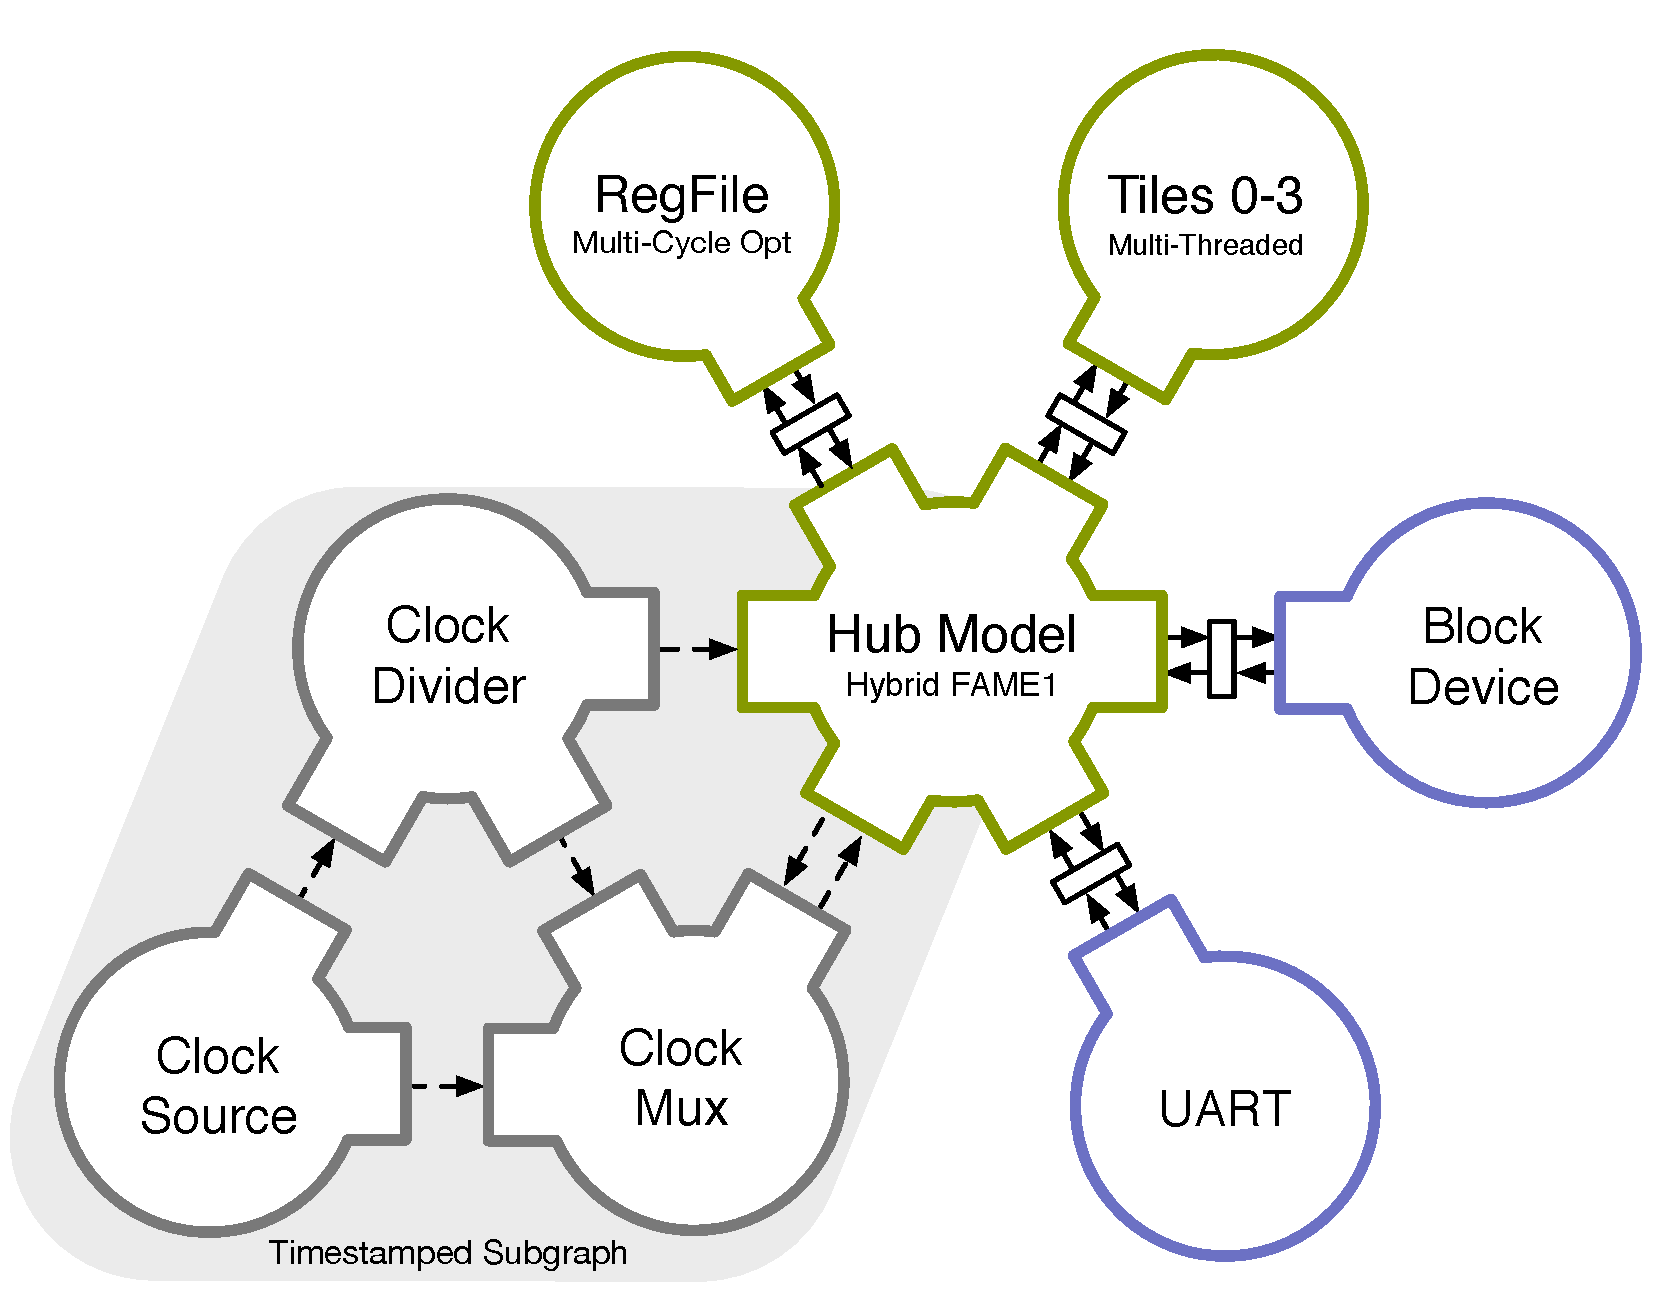
\includegraphics[width=0.99\textwidth]{figures/gg-graph-pdes.pdf}
    % NB: Bounding box of the timestamped subgraph screws up pdf whitespace
    % -c pdes midas-graphics/graffle/midas2-target.graffle figures/gg-graph-pdes.pdf
    \caption{An example simulator graph with a timestamped subgraph
    responsible for modeling clock generation.  Note, the ports represented in
    timestamped models are logical. The clock divider and clock mux both have a
    single output: output messages are duplicated and transmitted to each sink
    over separate channel.}
    \label{fig:gg-graph-pdes}
\end{figure}

For this approach to have acceptable performance, we needed to permit TUs to
send messages directly to one another, instead of forcing these transmissions
to propagate through the hub.  To do so, we introduced a compiler optimization
that removes passthrough connectivity in the hub, permitting two units
(timestamped or untimestamped) to drive each other directly. As a result,
simulator graphs are no longer guaranteed have a star topology (this is
visible in Figure~\ref{fig:gg-graph-pdes}).  While essential for the prototype
described here, this optimization also improves FMR in designs described in
previous chapter when multiple optimizations are enabled. We expand on this
optimization and other compiler modifications in Section~\ref{sec:pdes-compiler-modifications}

Since there is no longer a clock token stream, we modified the hub unit to
schedule across multiple timestamped inputs. Timestamped inputs can be either
clock-type or data-type~(used for modeling asynchronous resets), these differ
in how they are presented to target RTL. The hub unit explicitly tracks target
time, which it uses to populate the timestamps of output messages as it advances.
We expand on the hub-unit modifications in Section~\ref{sec:pdes-hub-modifications}.

To reiterate, TUs are implemented as bridges that use timestamped channels
exclusively. From the RTL designer's perspective, they are employed no
differently than conventional bridges in the target design.  However, writing
TUs that were both correct (deterministic, deadlock free, and timing exact) and
performant we found to be the most challenging aspect of our approach.  To ease
this process, we wrote a Chisel library of timestamped circuit primitives to
make it possible to write simple TUs as translations of verilog RTL.
Unfortunately, these primitives are conservative and cannot exploit lookahead
that might emerge in their composition. We describe these baseline TU
implementations in Section~\ref{sec:pdes-baseline-units}.

\subsection{Simplifying Assumptions}\label{sec:pdes-assumptions}

Perhaps the most attractive aspect of our approach is that it imposes few
restrictions on what a TU models. If the behavior of an extracted circuit can
be captured expressed as a 2-state value-change dump~(VCD), it is possible to write a
TU that matches that behavior. However, some new complexities arise when
considering interactions that span timestamped and untimestamped regions of the
simulator where the SSM assumptions still holds. In our initial prototype, we
make the following assumptions:

\begin{itemize}

\item Untimestamped channels remain synchronous in that they observe the hub only on
    positive edges of their associated clock and once at time zero. For example,
    if the input to a unit is driven by asynchronously reset state the sink
    unit will never see a token launched by the assertion of that reset. If these transitions must be modeled
    with sub-cycle accuracy a TU must be used.

\item All clocks must sourced by TUs. Clocks cannot be generated in
    FIRRTL with type casts from other data types.

\item All stateful target hardware in the hub or in UUs must be
    positive-edge triggered. While this restriction can be easily relaxed in
    the future, for the time being level-sensitive and
    negative-edge-triggered\footnote{This can also be achieved by replacing
    these elements with positive-edge triggered equivalents driven by an inverted
    clock.} hardware should modeled in TUs.

\end{itemize}

\subsection{Target-Side User Interface}

From the user's perspective, TUs are bridges.
The user annotates a clock-generating module with a \texttt{BridgeAnnotation},
and divides its target-side interface into channels. The bridge annotation
calls out a specific \texttt{BridgeModule} class the implements the desired
timing model. In Listing~\ref{lst:timestamped-bridge}, we show an example of
how we expect TUs to be deployed, using our library implementations of a clock
multiplexor and divider as examples.

\vbox{
\begin{lstlisting}[language=Scala, style=scalaStyle,
label={lst:timestamped-bridge}, caption=An example of the target-side modifications required to call out clock-generating primitives as units.]
// The existing clock divider module instantiation
val clockDivider = Module(new rocketchip.util.ClockDivider2)
clockDivider.io.clk_in := fullRate
val halfRate = clockDivider.io.clk_out

// Annotate the divider indicating it can be replaced
// with a TU. This is a strict addition, and requires
// no other modification to the design

BridgeableClockDivider(
  // The first parameter provides the module
  clockDivider,
  // Successive parameters provide the mapping
  // from target signal to timestamped channels
  clockDivider.io.clk_in,  // Input
  clockDivider.io.clk_out, // Output
  // The BridgeModule's constructor parameter
  div = 2)

// A similar example, using a clock mux
val clockMux = Module(new testchipip.ClockMux2)
clockMux.io.clocksIn(0) := fullRate
clockMux.io.clocksIn(1) := halfRate

// Annotate the clock mux, as above
BridgeableClockMux(
  clockMux,
  clockMux.io.clocksIn(0),
  clockMux.io.clocksIn(1),
  clockMux.io.clockOut,
  clockMux.io.sel)
\end{lstlisting}
}

\subsection{Message Representation and Channel Design}~\label{sec:messages}

In our system, signal that spans two TUs is represented with a trace of messages, each labeling a transition
with the time at which it occurs. This defines in effect, a two-state VCD
for the signal.  While there are many ways to optimize message encoding (much
like there are many ways to compress a VCD), logically all messages in our
system have two fields: a timestamp, which is a 64-bit unsigned integer
representing an absolute time in a simulator-global timebase, and data, which represents the value of the signal
at the associated time.

For a concrete example, consider a clock. A clock-type message consists of the
64-bit timestamp and a boolean data field. To represent the clock over the
duration of a simulation, a source must send a message on every transition, so to encode $N$ periods
the source must send at least $2N$ messages.  We say ``at least", because we
rely on the Chandy-Misra-Bryant~\cite{NullMessagesBryant} deadlock-avoidance
algorithm, and so practically speaking, many message streams will include null
messages. In our implementation, a null message shares the same data value as
the most recently sent message but with a later timestamp.

In our initial implementation, all timestamped channels are implemented with a single fully decoupled queue.
This means they can transmit at most (i.e., enqueue
or dequeue) a single message per host cycle. Without further optimization, this
implies that simulator FMR has a lower bound of two, since any unit processing a
clock-message stream must handle a negative-edge transition in every other
cycle. While there are many approaches that can overcome this limitation, which
we discuss in Section~\ref{sec:pdes-future-work}, in this chapter we work within
this simple but general representation.

\subsection{Correctness Of Logical Processes}\label{sec:lp-correctness}

In their paper, Chandy and Misra~\cite{NullMessagesChandy} provide a formal
specification of their null message-based conservative PDES and define its correctness vis-a-vis the
physical system it simulates. We provide a informal, english language summary
here.  As we introduced in Chapter~\ref{sec:fpga-des}, a physical system
consists of graph of communicating physical processes. In our systems,
physical processes are digital circuits, of any scale, that communicate by
driving wires that connect them.

To reason about the correctness of TUs (really, LPs), much like LI-BDNs,
we must frame them against output traces generated by their references (PPs).
Chandy and Misra refer dub the sequence of all messages sent from source
$i$ ($PP_{i}$) to sink $j$ ($PP_{j}$) up until time $t$, as a message \emph{history},
$h_{ij}(t)$.  LI-BDN's have an analogous definition of history: their
``messages" simply lack explicit timestamps, and $t$ is specified in cycles.
In the logical system, the message history between the equivalent source and
sink LP is given by $H_{ij}(t)$, where analogously,  $H_{ij}(t)$ is the
sequence of messages sent from $LP_{i}$ to $LP_{j}$ up until time $t$. Crucially,
$H$ and $h$ differ in that $h$ can never contain null messages: these are an
artifice of the the simulation required to avoid deadlock.

Chandy and Misra say a message history between a source and sink LPs is
\emph{correct} if and only if all messages of $h_{ij}$ are present in $H_{ij}$,
and every message in $H_{ij}$ either exists in $h_{ij}$ or is a null message.
In simpler terms, rejecting all null messages in $H_{ij}$ should produce $h_{ij}$,
or in an engineer's terms, rejecting all null messages should yield the VCD for
the wire that connects the PPs. This gives a concrete means to verify a
TU against a piece of reference RTL: pass identical inputs (i.e., $H$
for this input is ``correct" in the sense above) to the reference module and the
TU and compare the (2-state) VCD of the reference RTL against the output
message history of the unit by removing all null messages.

\subsection{Hub Unit Modifications}\label{sec:pdes-hub-modifications}

At a high-level, the primary change to the hub-unit is the introduction of a
frontend to the pipeline that reconstitutes the clock token from a set of
timestamped inputs. Timestamped inputs are processed in two groups, base on the FIRRTL type of their target signals:

\begin{itemize}

\item \textbf{Clocks:} These drive FIRRTL \texttt{clock}-typed inputs. As mentioned in Section~\ref{sec:messages},
these are timestamped booleans. On a positive-edge transition, a dedicated clock buffer
responsible for driving the target clock is enabled.

\item \textbf{Data:} These drive any FIRRTL non-clock ground-type including
    \texttt{UInt}, \texttt{SInt}, and, notably, \texttt{AsyncReset}. Updated
        values are presented to the target RTL by latching new values into a
        register at the times indicated in the message stream. In this way, an
        asynchronous reset transition can be presented at time when no clocks
        are active, and timestamped outputs can observe newly launched transitions in distinct messages.
\end{itemize}

\begin{figure}
    \centering
    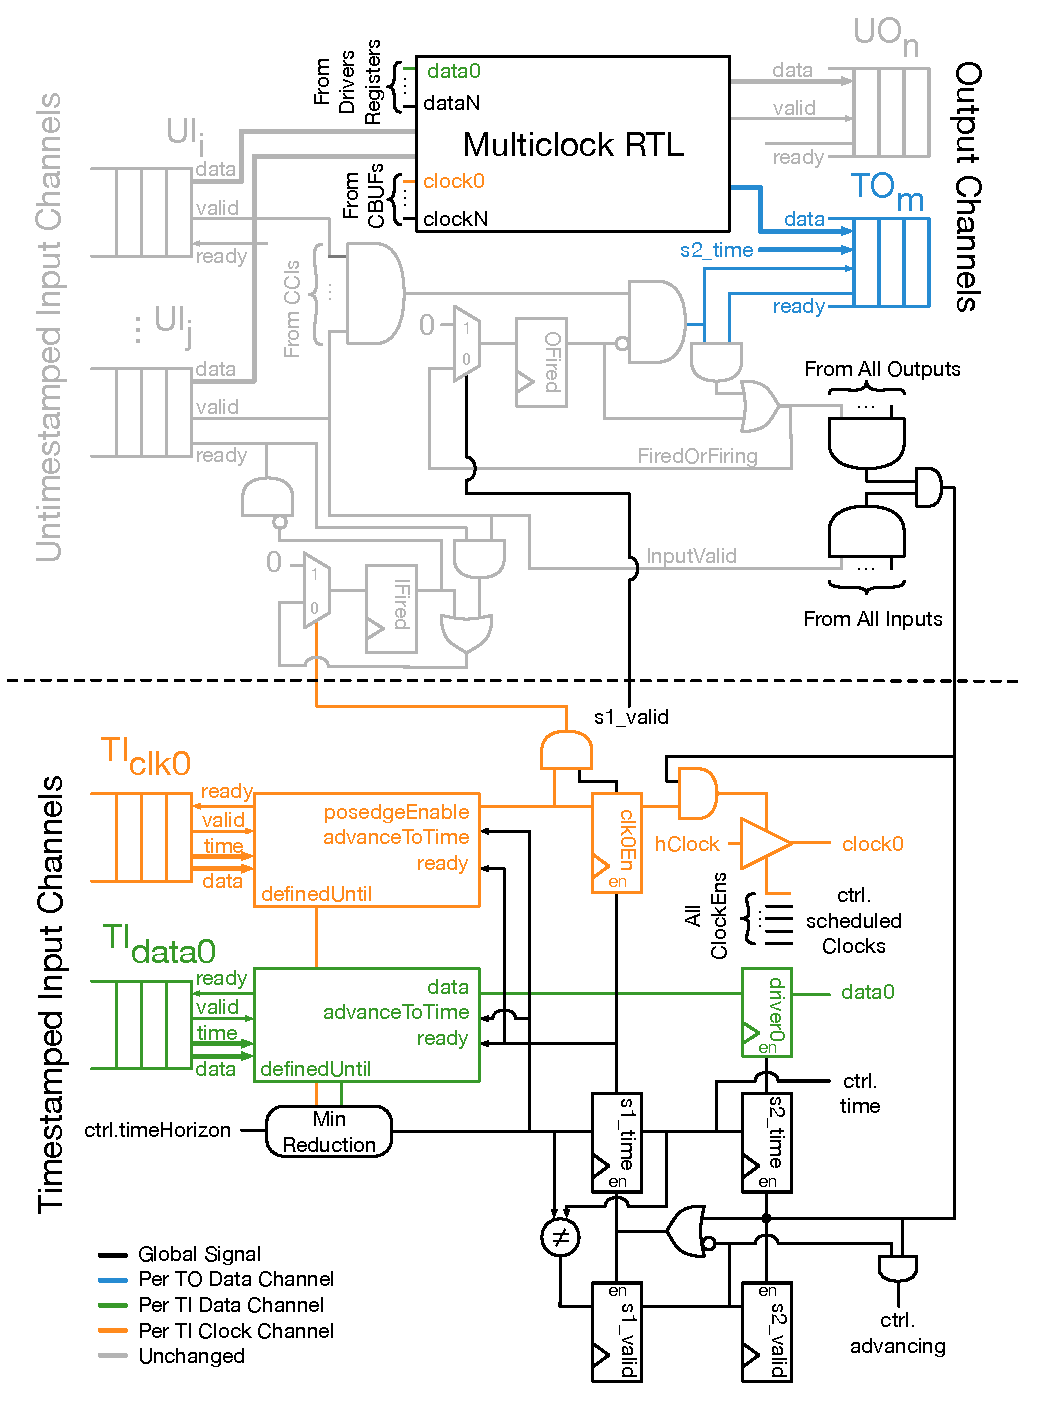
\includegraphics[width=0.99\textwidth]{figures/pdes-wrapper.pdf}
    % graffle2pdf -c pdes-wrapper midas-graphics/graffle/wrapper-transforms.graffle figures/pdes-wrapper.pdf
    \caption{The updated hub-unit wrapper. Circuitry in grey is unchanged from the multi-clock
    wrapper we showed in Figure~\ref{fig:static-multiclock-wrapper}}.
    \label{fig:pdes-wrapper}
\end{figure}

We show the updated hub unit in Figure~\ref{fig:pdes-wrapper}. The frontend
of the control pipeline~(bottom) consists of a series of decoders that
unpack messages to provide the horizon over which an input is
defined~(\texttt{definedUntil}) and detect transitions.  If an input message
produces a transition it is not dequeued: the decoder sets
\texttt{definedUntil} to that message's timestamp and waits. Conversely, null
messages and negative-edge transitions in clock-type channels are dequeued
upon arrival, which allows that input's horizon to advance further. When no message is available,
the decoder holds \texttt{definedUtil} at the timestamp of the last message.

With the inputs unpacked, the frontend performs a minimum-reduction across the horizons of all timestamped
inputs and an upper bound provided through the control
interface~(\texttt{ctrl.timeHorizon}).  This becomes the candidate time for the
next timestep and is broadcast back to each
decoder~(\texttt{advanceToTime}).  If the pipeline can advance, all decoders
with a transition or positive clock edge at the scheduled time dequeues their
input messages, and has their updated signal value latched.  The concatenation of all
enabled positive edges (\texttt{posedgeEnable}) corresponds to a clock token in
the sense defined in the previous chapter. Note that it is possible for there to exist no
transitions in a given timestep, it is scheduled anyway for reasons we will
discuss momentarily.

The ``clock token" and data updates are scheduled and flow through the pipeline
as in the previous chapter (note, the first stage of the pipeline for data values is absorbed into the scheduler).
Untimestamped input~(UI) and output~(UO) channels handling
has not changed, their control FSMs are only reset when their clock has been
scheduled to fire. One critical implication of this is that asynchronous events
launched by data-type transitions in a particular domain do not launch new
tokens in an untimestamped channel. This is consistent with our previous
assumption from Section~\ref{sec:pdes-assumptions}, that untimestamped channels
only observe outputs synchronously with respect to their associated clock.

Timestamped outputs are managed differently. To avoid certain deadlock
conditions, TOs generate a new message on every timestep,
notably those in which no clock or data transitions have been scheduled. In
effect, these outputs have their FSMs reset on every timestep~(via \texttt{s1\_valid}), and source their
timestamp from the pipeline~(\texttt{s2\_time}).  Without further
optimization, this baseline hub unit guarantees that output channels will
always be defined only as far as it oldest timestamped input.  Critically, this
means the hub unit has zero lookahead. Thus to avoid deadlock,
any arc of TUs that begins and ends at the hub must provide non-zero lookahead.

To provide finer-grained control and instrumentation, the hub exposes specific
signals to a memory-mapped simulation controller. This controller can detect
whether clocks are scheduled to fire~(\texttt{ctrl.clocksActive}), the time of
the associated timestep~(\texttt{ctrl.time}), and is responsible for setting
the time upper-bound~(\texttt{ctrl.timeHorizon}) past which the hub must not
advance.

\subsection{Compiler and Annotation Modifications}\label{sec:pdes-compiler-modifications}

\begin{figure}
    \centering
    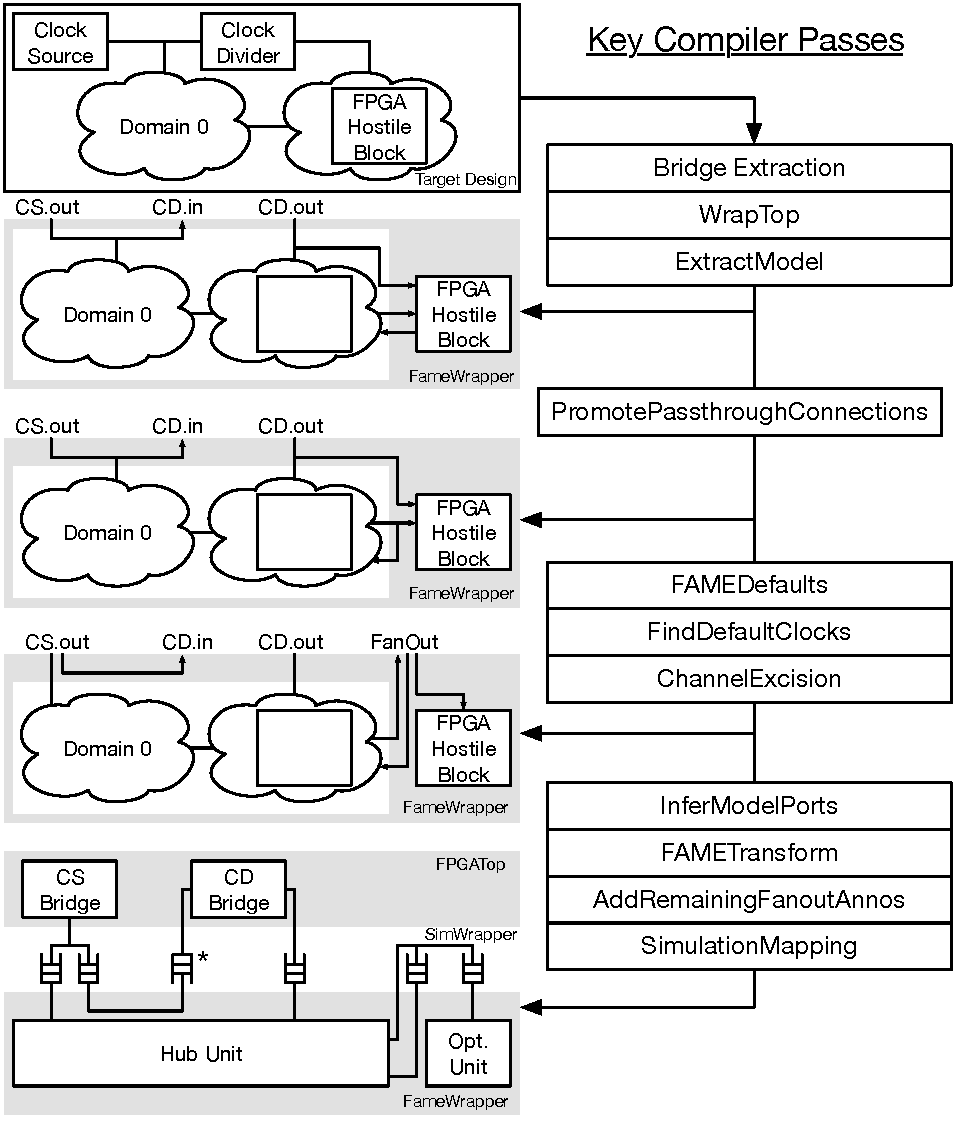
\includegraphics[width=0.99\textwidth]{figures/promote-passthroughs.pdf}
    % graffle2pdf -c main midas-graphics/graffle/promote-passthroughs.graffle figures/promote-passthroughs.pdf
    \caption{A visualization of the promote passthrough optimization.
    Modifications to the target are shown on the left at key points during
    compilation. We include a passthrough path in a optimizable block (right)
    to show how this transformation is broadly applicable to all inter-unit
    connectivity. Note, there is an extra channel generated (asterisk) in the
    bridge-to-bridge case currently, this can be optimized away in a future change.}
    \label{fig:promote-passthroughs}
\end{figure}

At first blush, baseline support for timestamped channels is relatively
straightforward to implement. Since all timestamped channels are wire-type, the
timestamp of a message can be treated as target data in an otherwise conventional
token, and wiring between channels and bridges can be left unchanged. However,
to provide a workable baseline implementation, we needed TUs to be
directly connected to one another, and not indirectly through the hub.  This
permits TUs to advance ahead of the hub unit (which in its current form has zero lookahead).
Our earlier assumption that only TUs
can source clocks and signals that launch asynchronous events lets us ensure that sources are only
ever directly connected to their sinks (~i.e., through a series of FIRRTL
\texttt{Connect} statements). This in turn simplifies the process of finding and extracting these
paths into point-to-point channels between two units. We refer to this enhancement
as the \emph{passthrough connections optimization} and give a pictorial representation of the process in Figure~\ref{fig:promote-passthroughs}.

The core of this change revolves around the
\texttt{PromotePassthroughConnections} transform, which extracts wires of any FIRRTL type that
passthrough any top-level SSM. We run this pass in target transformation, after bridge and model extraction.
Note, if a signal drives no other sinks aside from output ports, we leave the
connection to the original unit in place instead of removing the connectivity altogether.  This
simplifies connectivity analyses that occur later in the compiler, and ensures
that all clocks still drive the hub (even if all of the state for a particular
domain has been extracted).

At this point top-level connectivity in the design now includes fanouts. To
handle this new class of connectivity we modified \texttt{ChannelExcision}. In
general, a fanout of $n$ produces one output interface, and $n$ input interfaces
(sunk by the hub unit and optimized models) on the FAMEWrapper~(see the
right-most fanout in Figure~\ref{fig:promote-passthroughs}). The resulting
channel annotations share the same \texttt{source} targets, but their \texttt{sink} targets point at unique
inputs.

While a model-driven fanout can be deduced by looking for matching source fields in
channel annotations, this does not apply to a bridge-driven fanout, since
bridge-driven channels leave their \texttt{sources} field empty.  Since
bridges are already removed (they are interfaces on the FAMEWrapper), a
bridge-sourced fanout of $n$ produces $n$ inputs and no output interfaces. The clock-source-driven interface (CS.out) in
Figure~\ref{fig:promote-passthroughs} is an example of this.
To re-associate these inputs with a single source, we collect bridge-driven
sources in fanout annotations~(\texttt{FAMEChannelFanoutAnnotation}). This
allows simulation mapping to drive the correct set of input interfaces from the
same bridge source. For consistency, we emit the same annotations for
unit-driven fanouts~(\texttt{AddRemainingFanoutAnnos}).

%differences between bridge vs model connectivity, added unneeded complexity by
%handling bridges like models, and promoting their black-boxes into the
%FAMEWrapper instead of completely extracting them\footnote{This is a vestige of
%transtioning from MIDAS endpoints to Bridges}, which could happen later in the
%compiler. Here

Since this optimization now removes passthrough clock paths in extracted SSMs,
an SSMs's target clock will be driven not from the hub, but instead from a TU-driven
input (the path from CD.out to the FPGA hostile block in
Figure~\ref{fig:promote-passthroughs}). This required a modification to
\texttt{FindDefaultClocks} to infer the clock fields of intra-UU channels by
finding a clock sink port on the hub that shares the same source as the clock
sink on the extracted SSM. This works because, as we previously suggested,
\texttt{PromotePassthroughConnections} ensures that all clocks remain driven to
the hub.

The final necessary change for this optimization was to generalize the
\texttt{FAMEtransform}'s re-wiring of the FAMEWrapper, which previously relied
on the assumption that all channels had to be sourced by a unit and sunk by a
top-level interface (or vice versa). Now inter-unit connectivity, like the
connection between the CS and CD in Figure~\ref{fig:promote-passthroughs}, must
also be rewired.

The optimization, while critical for the implementation of this dissertation
work, can improve FMR in simulators without a timestamped subgraph notably when
using multi-cycle optimizations inter-model or bridge-to-model, paths need not
propagate through the hub model first. In a target in which a passthrough path
would winds through the hub, through an extracted model, and back to hub (with
no other combinational paths that span the same arc), FMR improves from a
best-case of three to two. This improvement becomes more pronounced for paths
that run through a cascade of connected models. This was the first major
contribution of the work of this chapter back to mainline FireSim (the
optimization is available in version 1.12).

\subsection{Baseline Timestamped Units}\label{sec:pdes-baseline-units}

Beyond a doubt, writing TUs was the most difficult aspect of building out our prototype.
Many of the aforementioned difficulties associated with
writing UUs apply, however TUs
must not only robust against changes in message arrival times (latency
insensitive), but they must be able to tolerate the presence of additional null
messages. In UUs, the designer must manage cycle-scale decoupling (for
example, that the output has advanced some number of cycles ahead of the
input), whereas in TUs this decoupling is considerably
finer-grained. Additionally, whereas SSMs without combinational loops have well defined
outputs for a given input trace, this is not true of many of the circuits we
wish to model here. One typical example of this is that there can often be
race conditions in standard Verilog implementations of these circuits that arise in due to the simultaneous arrival of inputs.
This can produce non-deterministic simulation behavior that is still is
compliant with Verilog's event-ordering model. Since determinism is
critical for making FireSim simulations debuggable, the TU designer is forced to pick a
behavior. Finally, TUs must extract sufficient lookahead from their
reference RTL to avoid deadlock and provide good simulation performance.

We built our baseline TUs using a modular approach that would make it easy to
rewrite verilog implementations as TUs. Specifically, we built a library of
timestamped utilities to manage and unpack message streams, circuit primitives
for registers, single-output combinational logic functions, and fanouts. For
each of these primitives we wrote deterministic Verilog reference
implementations, and built timestamping hardware capable of translating the
reference output into a message stream. This let us compare TU outputs with
reference-generated message traces as part of a dynamic verification flow.

A key limitation of these initial implementations is that they omit
asynchronous reset. While not insurmountable, asynchronous reset poses a key
challenge to our approach as it tends to remove lookahead opportunities afforded
by target state. In lieu of this, we rely on FPGA programming or host reset put
TUs in desired initial state.  We discuss the complexity of modeling asynchronous
reset in these TUs in Future Work~(Section~\ref{sec:pdes-future-work}).

\subsubsection{Timestamped Tuples: Unpacked Messages}
Message streams are difficult to directly act upon, as in general, we are often interested
in data values between messages. One reasonable approach is to insert incoming messages into a
age-ordered event queue (as a software implementation would) and update TU state in message order.
In our TUs we went with a distributed approach, in which we wrote ad-hoc state machines to schedule over per-input
datastructures to avoid serialization on a single event queue.
Given our baseline message encoding it is not possible to
detect transitions in a signal without comparing it an older value, so these
hardware datastructures, which we refer to as \emph{timestamped tuples}, ease
this process by holding hold a pair of messages: the latest message (the head
of the channel's queue), and the previous message. When a unit wishes to
process events created by a non-null input message, it asserts \texttt{observed},
which moves the latest message into the secondary slot and the next message in
the queue becomes visible. At the point the former \texttt{previous} message is no longer visible,
and cannot affect output messages and internal state changes.

Unlike early conservative PDES work, in which lookahead in an LP is statically
defined, our TUs can dynamically extract lookahead based on the values of
currently visible inputs. This is a domain-specific optimization akin to that
first described by D. Nicol~\cite{ImplicitLookahead} and B.
Lubachevsky~\cite{ImplicitLookahead2}. To describe lookahead properties of our
library primitives, it is useful to define variables that derive simply
timestamped tuples. Suppose we have an input $I$, we define:

\begin{itemize}
    \item $T_{I}$ to be the time of the latest message. We refer to this as the \emph{horizon} of $I$.
    \item $P_{I}$ to be the time of the previous message.
    \item $I_H$ to be the data value of $I$ at its horizon.
    \item $I_P$ to be the data value of $I$ before its horizon, and defined at least as far as $P_I$.
    \item $I(t)$ to be the data value of $I$ at time $t$, where:
\end{itemize}
\[ I(t) = \begin{cases}
    I_H & \quad \text{if } t = T_{I} \\
    I_P & \quad \text{if }  T_{I} > t \geq P_{I} \\
    undefined & \quad \text{otherwise} \\
\end{cases}
\]

Generally speaking, lookahead is defined with respect to the oldest input
received by an LP. In many of our TUs, lookahead will be zero notably when a
clock lags lags all other inputs. However, this may be permissible if the the
clock input is not part of a cycle in the timestamped subgraph, or if at least
one other TU in a cycle containing this input has non-zero lookahead. As we
will see, of particular concern for deadlock avoidance are hub-driven control inputs to TUs. Here, we
define \emph{relative lookahead}, which is the available lookahead in a TU,
when a specific input lags all other inputs. For example, select-relative
lookahead on a clock multiplexor refers to the lookahead available when the
select input to the mux lags all clock inputs.

\subsubsection{Edge-Triggered D Flip Flops}
D flip-flops, both positive and negative-edge triggered, are critical elements
for building integer clock dividers and clock multiplexors. Our basic
timestamped model has three compile-time parameters: the chisel type the
register stores, the initialization value register assumes at time 0, and
flip-flop's edge sensitivity.  Structurally, it has a clock-type input, and a
data-type input (D) and output (Q) of the data type above.  This primitive
models no clock-to-Q delay, and so an output transition on Q occurs
simultaneously with a latching edge. Additionally, this register observes the value of D one
timescale unit before the positive edge. Thus, if a clock and data transition
occur simultaneously, the clock always observes the old value of D.  This is
often a data-race in a Verilog expression of a flip-flop as the assignment to D
and the evaluation of RHS of a non-blocking assignment to Q can be executed in
either order. Our implementation ensures the non-blocking RHS evaluation occurs
first. We give the rules governing the timestamp of an output message based on
the available inputs, and thus the available lookahead ($T_L$) below:

\begin{algorithmic}
    \If {$T_{clock} \geq T_{D}$}
        \If {$\text{Clock} = \text{latching edge} \textbf{ and } (T_{clock} - T_{D}) > 1$}
            \State $t_{L} = (T_{clock} - 1) - T_{D}$
        \Else
            \State $t_{L} = T_{clock} - T_{D}$
        \EndIf
    \Else
        \If {$D_H = Q_H$}
            \State $t_{L} = T_{D} - T_{clock}$
        \Else
            \State $t_{L} = 0$
        \EndIf
    \EndIf
\end{algorithmic}

Using the information encoded in the message streams alone, this register's
output cannot always advance ahead of both Clock and D. However, it does have non-zero D-relative lookahead, which will suffice to avoid
deadlock in many important classes of designs we will discuss in
Section~\ref{sec:pdes-common-circuit-perf}.  We note, the most natural way to
introduce clock-relative lookahead, if required, is to model a clock-to-Q
delay. Similarly, D-relative lookahead could be improved by having the model
observe D earlier relative to the clock edge, as the path will need to meet
a reasonable setup time constraint to avoid metastability.

\subsubsection{Generic Combinational Functions}
Our baseline utility to describe combination functions schedules over a set of
timestamped tuples, and generates a single output message at the timestamp of
the oldest input message. This is convenient in that the user can generate
arbitrary combinational logic over all input tuples, however it comes at the
cost of zero lookahead. Without providing additional hints about input transitions, there are two
mechanisms for finding more lookahead.  The first is modeling propagation
delays through gates. Here, $$t_L = \min_{\forall I} (T_{I} + minPD_{I})$$
where $minPD_{I}$ is the minimum propagation delay of the circuit from input $I$ to
the output.  The second means is to leverage logic redundancy. If the oldest
input to a combinational function cannot not affect the output (i.e., it can be
treated as a don't-care) the output can advance ahead of that input.

\subsubsection{Fan Outs}
To broadcast a timestamped tuple from one source to many sinks, we wrote a fanout
primitive. Under-the-hood, this repacks the tuple into a message that is then
broadcast to a set of queues, much in the same way a fanout channel is
implemented in in the simulation wrapper. These queues are of finite depth, and
must be sized conservatively by the designer to avoid deadlock.

\subsubsection{Clock and Asynchronous-Reset Sources}

For use in test harnesses, we wrote primitives to act as idealized sources for
clocks and asynchronous resets.  Our clock source generates an infinite trace
of clock messages, and has a compile-time configurable period, initial value,
and duty cycle.  Having only a single clock output and no inputs, it
effectively has infinite lookahead and can run arbitrarily far ahead of other
TUs in the graph.  Similarly, our asynchronous reset source drives a pulse of
configurable length and polarity, after which it remains deasserted-asserted for the
remainder of simulation (a total of three messages). Both of these primitives
have wrapper bridge module, and so can be used in target RTL.

\subsubsection{Library Timestamped Units}
Using these library primitives we built simple TUs by translating verilog into
timestamped equivalents. We give an example of this using a phase-aligned,
by-two clock divider: its reference verilog is shown in
Listing~\ref{lst:verilog-clock-divider} and its timestamped translation is
shown Listing~\ref{lst:tu-clock-divider}. Using this scheme, we also wrote baseline
TUs for a by-three clock divider~(Figure~\ref{fig:by3-clock-div}), a glitchless
two-to-one clock multiplexor~(Figure~\ref{fig:clock-mux-glitchless}) and an
and-based, ICG~(Figure~\ref{fig:clock-gate}).  Note that the output clock in
each of these circuits is not combinationally dependent on a control input:
they all have non-zero control-relative lookahead.

\begin{lstlisting}[language=Verilog, style=verilogStyle, float,
label={lst:verilog-clock-divider}, caption=A reference phase-aligned clock-divider from Rocket Chip used in RTL simulation.]
module ClockDivider2 (output reg clk_out, input clk_in);

   initial clk_out = 1'b0;
   always @(posedge clk_in) begin
      clk_out = ~clk_out; // Must use =, NOT <=
   end

endmodule // ClockDivider2
\end{lstlisting}

\begin{lstlisting}[language=Scala, style=scalaStyle, float, label={lst:tu-clock-divider}, caption=The equivalent TU for the clock divider shown in Listing~\ref{lst:verilog-clock-divider} implemented using library primitives.]
class ClockDivider2 extends MultiIOModule {
  val clk_in   = IO(Flipped(new TimestampedTuple(Bool())))
  val clk_out  = IO(new TimestampedTuple(Bool()))
  val reg = Module(new TimestampedRegister(Bool(), Posedge, init = Some(false.B)))
  reg.simClock <> clk_in
  val Seq(feedback, out) = FanOut(reg.q, "feedback", "out")
  clk_out <> out
  reg.d <> (new CombLogic(Bool(), feedback){
    out.latest.bits.data := ~valueOf(feedback)
  }).out
\end{lstlisting}

\begin{figure}
    \centering
    \begin{subfigure}[t]{0.35\textwidth}
        \captionsetup{margin=0.25cm}
        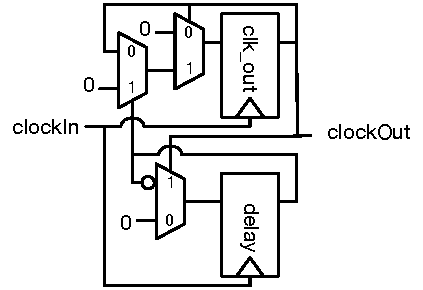
\includegraphics[width=\columnwidth]{figures/clock-div3.pdf}
        \caption{By-3 clock divider.}
        %graffle2pdf -c clock-divider-3 midas-graphics/graffle/clock-muxes.graffle figures/clock-div3.pdf
        \label{fig:by3-clock-div}
    \end{subfigure}
    \hspace{-1cm}
    \begin{subfigure}[t]{0.40\textwidth}
        \captionsetup{margin=0.25cm}
        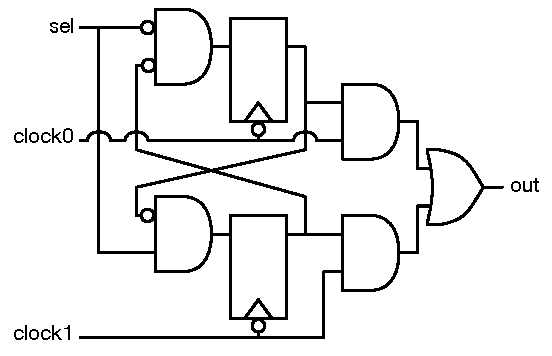
\includegraphics[width=\columnwidth]{figures/clock-mux-glitchless.pdf}
        \caption{Glitchless clock mux.}
        %graffle2pdf -c glitchless midas-graphics/graffle/clock-muxes.graffle figures/clock-mux-glitchless.pdf
        \label{fig:clock-mux-glitchless}
    \end{subfigure}
    \hspace{-1cm}
    \begin{subfigure}[t]{0.30\textwidth}
        \captionsetup{margin=0.25cm}
        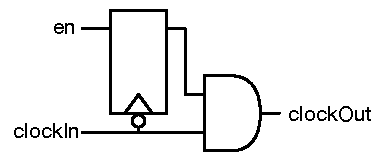
\includegraphics[width=\columnwidth]{figures/clock-gate.pdf}
        \caption{Clock-gating cell.}
        %graffle2pdf -c clock-gate midas-graphics/graffle/clock-muxes.graffle figures/clock-gate.pdf
        \label{fig:clock-gate}
    \end{subfigure}
    \centering
    \caption{Reference circuit diagrams for the baseline TUs. Verilog for the
    by-2 divider is provided in Listing~\ref{lst:verilog-clock-divider} so we
    omit it here.}
    \label{fig:baseline-reference-circuits}
\end{figure}

\subsection{Verification}

We relied on dynamic verification to check our implementations. We
wrote a SystemVerilog ``timestamper" which translates a signal into a decoupled
message stream, by leverage Verilog's \texttt{\$time} system function to
produce a timestamp. We then wrote chisel testbenches to show hat two message
streams were correct in the manner described in
Section~\ref{sec:lp-correctness}.
%We wrote fuzzers to inject both host-delays and additional null messages into message streams,

As we have mentioned, many of the aforementioned circuits have expected
non-deterministic behavior when written in a conventional Verilog style. To
ease verification, we wrote race-free reference implementations which guarantee
a particular ordering by judiciously adding sub-\texttt{time\_unit} delay to
statements in the reference. This approach does not scale to compositions
of these circuits, but suffices to verify small circuits are
deterministically represented by its TU.

\section{Performance in Common Clock Organizations}\label{sec:pdes-common-circuit-perf}

\begin{figure}
    \centering
    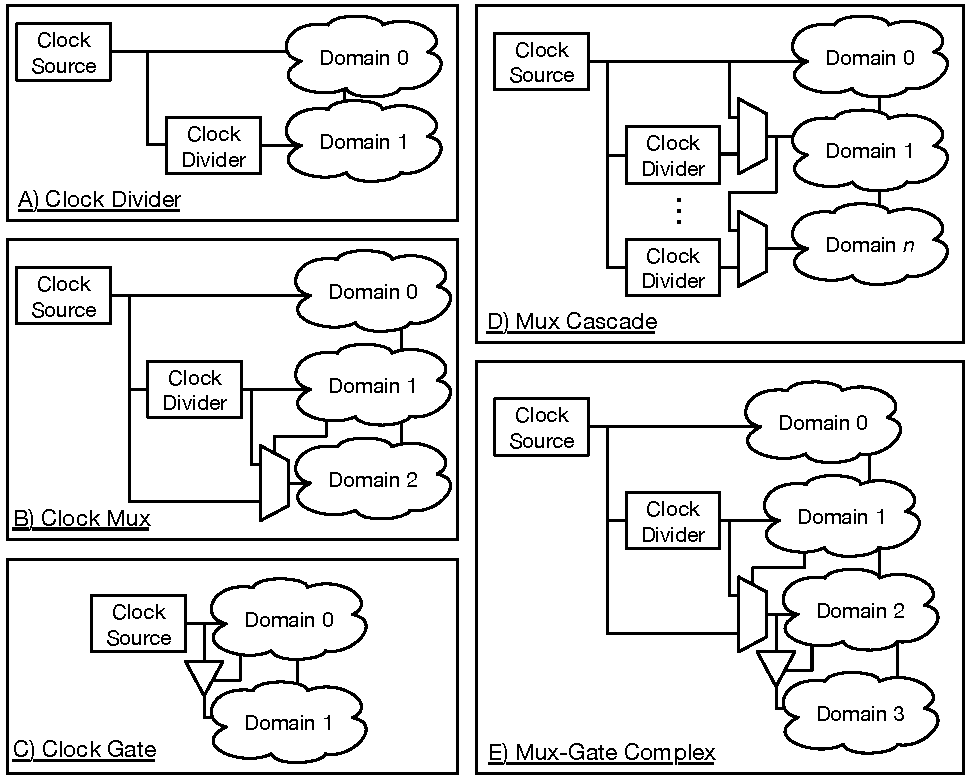
\includegraphics[width=0.99\textwidth]{figures/clock-organizations.pdf}
    % graffle2pdf -c combo midas-graphics/graffle/clock-organizations.graffle figures/clock-organizations.pdf
    \caption{Five illustrative clock organizations that leverage each of the TUs we have built.}
    \label{fig:clock-organizations}
\end{figure}

What should be clear from the previous sections is that these baseline TUs are
conservative. Since they make no assumptions about the behavior of their
inputs, they cannot find lookahead in all of their input corners, specifically
in cases where a clock-type input is oldest input to the unit. Fortunately, in
many useful classes of clock organizations (depicted in
Figure~\ref{fig:clock-organizations}), there are no cycles that do not span the
hub unit. Since all of our TUs have non-zero relative lookahead with respect to
their hub-driven inputs---which are necessarily data-type---all of these circuits narrowly avoid deadlock.
Of course, this does not imply that the resulting simulator is performant: here we measure
the FMR of our prototype simulating the circuit organizations of
Figure~\ref{fig:clock-organizations}, and shed light on the origin of
performance losses where they exist. We summarize the FMRs of these circuits in
Table~\ref{tbl:pdes-baseline-fmrs}.

\begin{table}[t]
\centering
    \begin{tabular}{c c c c c}
    \hline
          \textbf{Divider} & \textbf{Mux} & \textbf{Gate} & \textbf{3-Mux Cascade} & \textbf{Mux-Gate} \\
          3.0 & 11.0 & 6.0 & (12.5, 13.0) & 15.5 \\
    \hline
    \end{tabular}
    \caption{Measured FMR of the clock organizations shown in Figure~\ref{fig:clock-organizations} using the baseline TUs.
    For the 3-mux cascade, we report the FMR when domain $i-1$ drives domain $i$'s
    clock select~(12.5), and when domain $i$ drives its own select (13.0).}
    \label{tbl:pdes-baseline-fmrs}
\end{table}

\subsection{Feedforward Divider Networks}

A feedforward network of clock sources and dividers
(Figure~\ref{fig:clock-organizations}, circuit A) is the simplest case, and
suffices to model the systems we described in the previous chapter. Performance
in these circuits is bandwidth bound on the ability of the downstream dividers
to process input messages from the high-frequency reference clock. The baseline
by-two clock divider, reported in Table~\ref{tbl:pdes-baseline-fmrs}, takes three cycles on average to process two input
messages (one reference clock cycle). This arises because the flip flop model, unaware
that it is driving itself in a feedback loop, waits for its D input to be defined one time unit
before the next positive clock edge, introducing a single internal null
message. Thus, when the fastest clock is driving other logic in the target, the
best case FMR of these targets is three.

It is important to note that if we remove the fast clock domain (domain zero in
Figure~\ref{fig:clock-organizations}), from the user's perspective the FMR
doubles to six~(when using by-two clock divider). Unfortunately, cases in which
the high-frequency clock is not widely deployed in the target-design is a
common case. For example, in order to generate the 1.5, 1.0, and 0.75 GHz
clocks for the three-domain target SoC we described in
Section~\ref{sec:spec-perf}, we would be forced to generate a 3.0 GHz
reference, and then use by-two, by-three, and by-four (two by-twos) clock divisions to generate
the target clocks. The cost of directly simulating the fast clock increases as
the ratio between the reference and the fastest derived clock grows. We
describe solutions to this problem in Section~\ref{sec:pdes-future-work}.

\subsection{Simple Hub Cycles}
ICGs and clock multiplexors (Figure~\ref{fig:clock-organizations}, circuits B
and C) create a two-unit cycle in the simulator graph that span a hub-driven
control signal and a TU-driven clock. Performance in these configurations is
latency bound on message transmission through this cycle and is further
deteriorated by null message transmissions that may require multiple serialized
trips through the cycle.

This is most clearly illustrated with the clock gate configuration, which has a
measured FMR of six. Both the reference clock and gated clock have the same
frequency, so there no new bandwidth bound introduced. Any additional slowdown is the
result of the ICG TU waiting on message propagation from the hub. We show this
process in Figure~\ref{fig:clocks-gate-control-loop}. In this example the reference clock
has a period of four, and a there is a positive edge at $t = 0$. Since the hub
must wait for input message from both the source and the ICG TU, and since the
ICG TU always lags the source, we neglect the source in this diagram.

There are two effects at play here. After the ICG has enqueued a positive-edged
message for its output clock at host cycle zero, it takes four cycles for a
enable message sharing that timestamp ($t = 0$) to arrive at the the TU's
input. A transition in enable would be visible in this message if it was to
occur. Unaware that it should expect no further transitions, the register model
in the ICG waits for an input defined one time\_unit before clock's negative
edge ($t \geq 1$). This requires a null message (the TU's second output
message) to propagate through the loop. Once it arrives at cycle five, the
negative edge is processed and the new enable value is latched. In host cycle
six, the second positive edge is finally enqueued. This cycle recurs thus
giving an FMR of six.

\begin{figure}
    \centering
    \captionsetup{margin=0.25cm}
    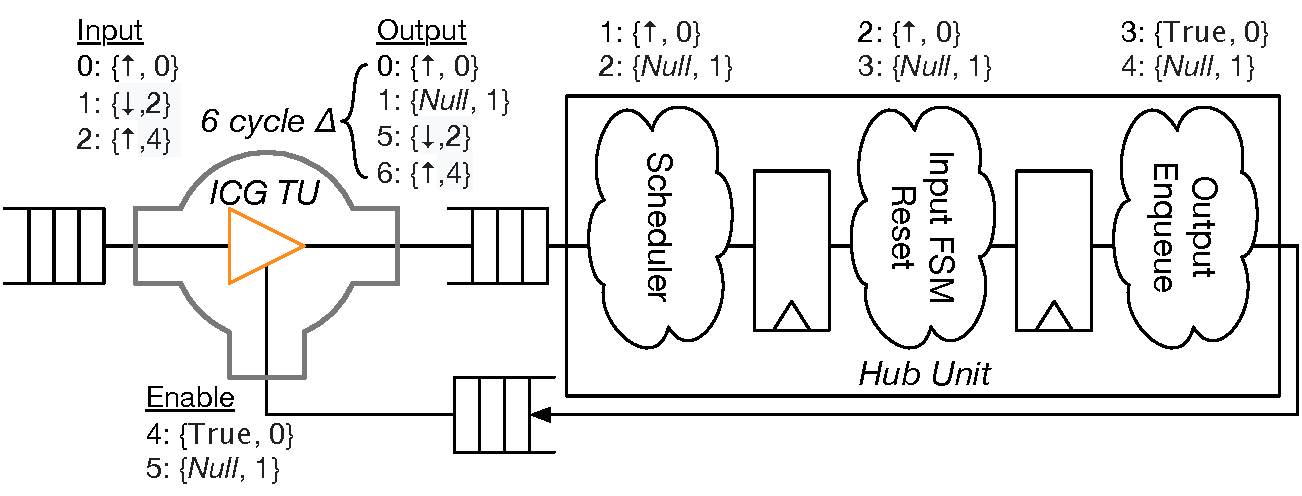
\includegraphics[width=\columnwidth]{figures/clock-gate-control-loop.pdf}
    \caption{An illustration of the clock gate configuration's measured FMR of 6.0. Messages are labeled
    \emph{host cycle}: \{\emph{data}, \emph{time}\}.}
    %graffle2pdf -c baseline midas-graphics/graffle/clock-gate-control-loop.graffle figures/clock-gate-control-loop.pdf
    \label{fig:clock-gate-control-loop}
\end{figure}

The clock multiplexor configuration has significantly worse FMR~(11.0) because null message propagation loops
are not always overlapped with the propagation of an edge (as in the previous
example). In other words, a null message received on the select input by the multiplexor launches a new
null message that must propagate through the simulator, instead of allowing the
unit to enqueue a new output edge.

\subsection{Multi-Unit Cycles}
Multiplexor cascades (Figure~\ref{fig:clock-organizations}, circuit D) and
multiplexor-gate complexes (Figure~\ref{fig:clock-organizations}, circuit E) are also
common occurrences in SoCs. Here a cycle exists starts at a hub-driven control
signal, passes through multiple cascaded TUs, and terminates at a clock input on the
hub. One might expect that these topologies would have greater FMRs, since the
transmission time across the loop is longer without extracting substantially
more lookahead per TU crossed.

This is not always case with multiplexor cascades when selecting between clocks
of the same frequency: it depends on which domain drives the select signal.
When the select is driven by the same domain the multiplexor drives, these
circuits run with an FMR of 11.0~(note shown) independent of the depth of the cascade ($N$).
When select is driven by the previous clock domain, FMR increases to 13.0.
When each stage is fed by a different frequency, for instance with clock
divider with a division of $i+1$, where $i$ is the index of the current domain,
the story becomes more complicated. Here increasing the cascade depth,
marginally increases FMR (12.5, 13.2, 13.2, from $N=3$ to $N=6$), due to the
introduction of new null messages by the dividers themselves. Removing these
messages would return FMR to 11.0.

Topologically, the mux-gate complex is analogous to the
previous-domain-drives-select mentioned in multiplexor-cascade example, as the
clock enable cannot solely be driven by state in the domain it is gating. Here we
measured an increase in FMR from 11 to 15.5 over the single multiplexor case, because
the launch of an enable message is serialized directly behind the selection of a
clock. Indeed, the primarily driver of increased FMR is not the length of a
cycle, which can be problematic, but rather tight coupling clock generation and
the control logic.

\subsection{Compositions Of Circuits}

We speculate that, in general, the circuits we present in
Figure~\ref{fig:clock-organizations} can compose with zero or modest increase
FMR if they derive from the same clock source, or from a second clock source
that is a phase-aligned integer division of the source. This is because their
message propagation happens in parallel, and few, if any, new simulator
timesteps are introduced. More complex compositions that derive from a clock
driven by a multiplexor require more detailed analysis, as which domains
drive control signals can have a large bearing on FMR. This effect is manifest
in both the mux-gate complex and multiplexor cascade circuits.

\section{Lookahead Optimized Units}\label{sec:pdes-opt-units}
While there are systemic approaches for improving simulation performance in our
initial implementation, the lowest hanging fruit revolve around optimizations
that can extract more lookahead in non-hub TUs. Without introducing logic or
propagation delay, this must rely upon leveraging the presence of state in the
reference circuits. This state provides a multi-period interval of
opacity~\cite{ImplicitLookahead2} wherein changes in the hub-driven control
signal are not observable in the output message stream---an effect we first
described in the context of channel-bootstrapped formalisms.
To this end, here we throw out the library primitives in favor of fully handwritten TUs.
The cost of this approach is that writing correct TUs becomes more challenging,
as these units cannot be simply transcribed from verilog.

\begin{table}[t]
\centering
    \begin{tabular}{c c c c c c}
           & \textbf{Divider} & \textbf{Mux} & \textbf{Gate} & \textbf{3-Mux Cascade} & \textbf{Mux-Gate} \\
    \hline
          Baseline        & 3.0 & 11.0  & 6.0 & (12.5, 13.0) & 15.5 \\
          Optimized Dividers   & \textbf{2.0} & 11.0          & ---        & (\emph{13*}, 13)             & 15.5 \\
          Optimized ICGs       & ---          & ---           & \textbf{4.0} &  ---                          & \textbf{14.0} \\
          Sync Mux, $k = 1$  & ---          & \textbf{2.6}  & ---        & (\textbf{3.0}, \textbf{4.8}) & \textbf{5.3} \\
          Sync Mux, $k \geq 2$ & ---          & \textbf{2.0}  & ---       & (3.0, 4.8)                   & \textbf{5.0} \\
    \hline
          All & 2.0 & 2.0 & 4.0 & (\textbf{2.0} \textbf{2.8}) & \textbf{2.7} \\
    \end{tabular}
    \caption{Measured FMR of the clock organizations shown in Figure~\ref{fig:clock-organizations} when introducing
    lookahead-optimized TUs. Bolded figures represent an improvement over the previous best. While previous rows
    substitute only a single type of TU to isolate FMR changes, the \emph{All} row uses optimized units exclusively.}
    \label{tbl:pdes-optimized-fmrs}
\end{table}

\subsection{Integer Clock Dividers}
If we continue to neglect asynchronous reset, it is trivial to write a
clock divider TU that can consume an input message per cycle. On
positive input clock edges, the TU increments a counter, and if the counter has
reached a threshold for a positive or negative output edge, it supplies the
appropriate output message.  Otherwise, the TU greedily enqueues output
null messages stamped to the arrival time of the last input clock edge.
Assuming an input message stream has no null messages, the only
circumstance under which this unit cannot process an input edge per host-cycle
is when there is output backpressure.

\subsection{Integrated Clock-Gating Cells}
A typical latch-based ICG is difficult to optimize because the latch
is transparent in the half-period directly before an input positive edge. As a
result, late arriving enable signals produce observable changes in the output.
Indeed, the latch exists to solely to prevent glitches in the output clock, so
from a lookahead perspective it is more illustrative to think of this circuit as
a combinational and of its inputs.  To avoid this, in our
primitive model, we used a negative-edge-triggered D flip flop instead of a
latch.

Without modeling new delays in the the TU, the only recourse the unit designer
has is to exploit knowledge about the behavior of the input message streams.
Here the main observation is that the clock-enable function tends to be
synchronous to the input clock.  If this is the case, and the enable signal is
being driven by the hub, there should eventually be an input message with the
same timestamp as the input positive edge that launched it.  Whereas the
baseline implementation must be sure the enable remains stable until the time of
the latching edge, in this case, the TU can lookahead one input cycle.
This removes the need to wait for null messages to arrive that ensure there are no
further changes in the enable. Referring to the FMR illustration for the clock
gate organization~(Figure~\ref{fig:clock-gate-control-loop}), this optimization
permits the ICG TU to enqueue the second positive edge on the same cycle the
enable message for the previous edge arrives~(note, the negative edge message
for the previous cycle would be enqueued on host cycle one).

\subsection{Clock Multiplexors}
%At their core, simple clock multiplexors~(Figure~\ref{fig:clock-mux-naive}) suffer from the same challenges as clock
%gates, with edges in the output clock being defined by a combinational function
%on the input clocks and select.
Our baseline clock multiplexor is based on the circuit in
Figure~\ref{fig:clock-mux-glitchless}, extracts the smallest degree of
lookahead available to avoid deadlock. While a handwritten model could do
better by exploiting knowledge of the feedback loop between the two
clock-select registers, to do better still, we can model multiplexors that produce observable changes
in the output clock many cycles after the select has changed~(they have a longer opaque period).
This is true of typical glitchless clock multiplexors designed to switch
unrelated clocks (Figure~\ref{fig:clock-mux-sync}), which we shall refer to as
a sync-multiplexor or sync-mux for short. Here the clock select must be first synchronized to each
clock domain, before it produces an observable change in the output
clock.

\begin{figure}
    \centering
    \captionsetup{margin=0.25cm}
    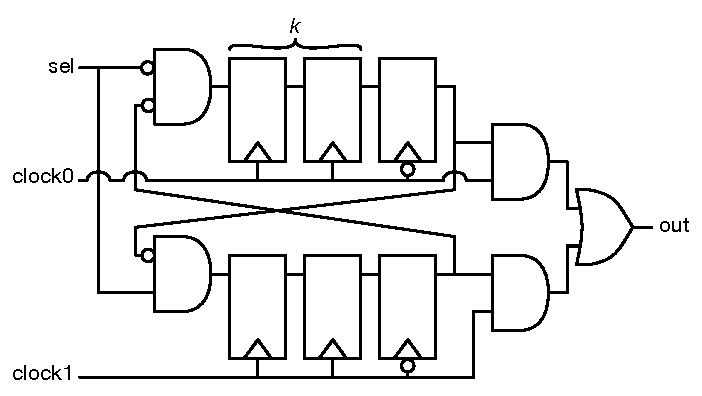
\includegraphics[width=0.6\columnwidth]{figures/clock-mux-sync.pdf}
    \caption{A synchronized, glitchless two-to-one clock multiplexor that can safely switch between two unrelated clocks.
    $k$ is the length of the synchronizer chain.}
    %graffle2pdf -c sync midas-graphics/graffle/clock-muxes.graffle figures/clock-mux-sync.pdf
    \label{fig:clock-mux-sync}
\end{figure}

We designed a TU unit to model this variety of clock multiplexor. Our
implementation is configurable in the number of input clocks ($n$), and the
depth of the synchronizer chain~($k$). Internally, this TU consists of $n$ clock handlers
which dequeue input messages up to $k$ positive edges in advance of
the select.  In steady state, a clock edge $k$ periods in the future of the
current clock select value can be driven to the output. On a transition no
further clock edges are presented. Instead, after a negative edge for currently
selected clock has been sent, the TU sends a null message corresponding to a
dead window of $k$ periods in the new clock domain. At this point, positive
edges for the newly selected domain are made visible as they arrive at the
clock handler. The choice of $k$ is the key determiner of the available
lookahead in this variety of multiplexor. In Table~\ref{tbl:pdes-optimized-fmrs} we
present FMRs for both $k = 1$ and $k \geq 2$ cases.  While the $k = 1$ case
already provides an enormous improvement over the baseline, it is typical to
set $k = 2$ or $k = 3$.  Under these configurations, the FMR cost of the
multiplexor is almost entirely removed.

\section{FPGA QoR And Scalability}

The feasibility of our approach hinges on the assumption that managing
large timestamps for relatively few and small TUs would incur a small resource
cost relative to the rest of the simulator. Here we quantify these costs by
measuring TU and hub-unit resource utilization and reporting their $f_{max}$.

% Vivado version

\subsection{TU Resource Utilization}
One would expect that building TUs that process multiple streams of messages
with large timestamps would bring about a large resource cost despite the
underlying simplicity of the target circuits they model. To collect these results for a given TU,
we elaborate a top-level wrapper circuit that registers all input and output
interfaces of the TU. We then used Vivado version 2018.2, with the default
synthesis and implementation strategies, to measure circuit QoR. To estimate
$f_{max}$ we over constrained the host clock in these designs to 200 MHz.

\begin{table}[t]
\centering
    \begin{tabular}{c c c c c}
        TU & Logic LUTs & Registers & Memory LUTs & $f_{max}$ \\
    \hline
        Clock Source & 38 & 63 & 0& 200 \\
        \hline
        ICG Baseline  & 1134 & 283 & 84& 128 \\
        ICG Optimized & 260 & 131 & 0& 200 \\
        \hline
        Clock Mux & 3372 & 1084 & 420& 164 \\
        Clock Mux (Sync, $k=3$) & 911 & 82 & 80& 200 \\
        \hline
        Divider (By 2) & 986 & 282 & 84& 200 \\
        Divider (By 3) & 2527 & 793 & 294& 153 \\
        Divider Optimized & 40 & 67 & 0& 200 \\
    \hline
    \end{tabular}
    \caption{TU resource utilization when targeting a Xilinx Ultrascale+ device (VU9P). We constrained our designs 200 MHz as that
    represents a substantial margin over typically realizable $f_{fpga}$.}
    \label{tbl:pdes-tu-utilization}
\end{table}

Table~\ref{tbl:pdes-tu-utilization} lays bare the reality the abstraction cost of the
library primitives used in the baseline implementations is significant. The largest
driver of utilization, in both optimized and baseline TUs, are timestamp comparisons. These occur in multiple places in the
baseline units, since each library primitive independently schedules across its
local inputs. Conversely, in the optimized ICG and clock multiplexor, this happens only
at the I/O boundary of the TU. Most starkly, since there is only a single input
to our clock divider TU, no timestamp comparisons are required: this produces
the large savings shown in Table~\ref{tbl:pdes-tu-utilization}. Nonetheless, as a fraction of the resources
available on the VU9P, TUs utilization, even in the unoptimized models, is
insignificant: the baseline clock mux uses 0.32\% of the VU9P's available LUTs,
whereas the optimized TU uses just 0.1\%\footnote{This is still an amusingly
large figure given that a fraction of single LUT is required to implement most of the
other 1-bit, 2:1 multiplexors in our simulators.}.
We suspect that using a more optimized message encoding and writing TU implementations that
avoid acting directly on absolute timestamps would suffice to make the cost of
the entire timestamped subgraph negligible in nearly all target systems.

TU $f_{max}$ is also acceptably fast. While some of the baseline units fail to
meet timing at 200 MHz, all of the optimized units do. 200 MHz is considerably
greater than the achievable $f_{fpga}$ of systems we typically simulate and
thus is unlikely ever adversely affect $f_{fpga}$.

\subsection{Hub Unit QoR and $f_{max}$ Scaling}
Another scaling challenge of our approach are costs associated with the
frontend of the hub unit's pipeline, which features a large minimum-reduction
across timestamps. We measured the per-timestamped-input scaling trends of the
hub by synthesizing a scan chain where each register is asynchronously reset
by an independent source. This adds a new timestamped input per register in the
chain while only using a single BUFGCE. Here we build complete
simulator bitstreams using FireSim's standard build flow with the ``timing''
strategy and Vivado version 2018.3.

\begin{figure}
    \centering
    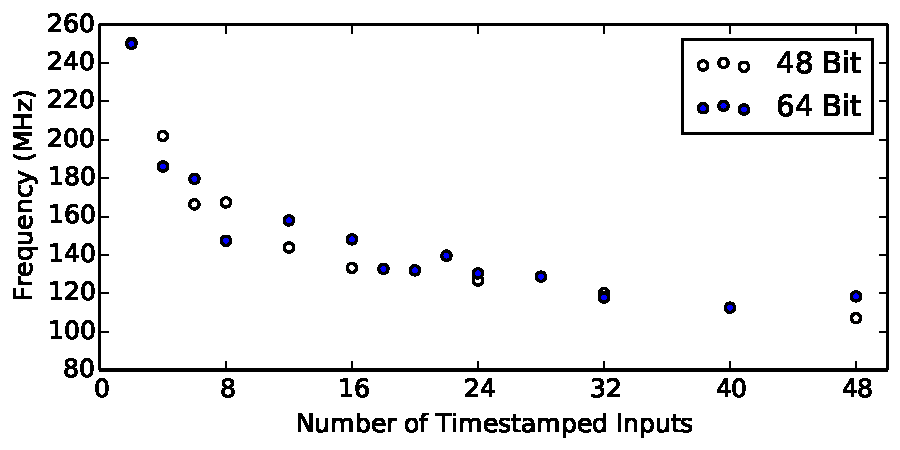
\includegraphics[width=0.75\textwidth]{figures/pdes--hub-fmax-scaling.pdf}
    \caption{Measured $f_{fpga}$ for simulators of 1-bit-wide scan-chain whose
    number of timestamped inputs is equal to the length of the chain plus one. Each
    point consists of a single design run. The underlying timing
    variability in FPGA implementation is evident with many 64-bit designs
    out-performing 48-bit equivalents.}
    \label{fig:pdes-hub-fmax-scaling}
\end{figure}

In Figure~\ref{fig:pdes-hub-fmax-scaling}, we plot $f_{fpga}$ of the simulator as
a function of the number of timestamped inputs used under both 48 and 64 bit
timestamps. To produce these numbers, we coarsely overconstrained $f_{fpga}$ (by up to 10 MHz in some cases). Given this
heavy-handed overconstraint and the inherently stochastic nature of FPGA place
and route especially when lacking placement constraints, fluctuations in $f_{fpga}$ are expected. The overall trend is clear
however. For both widths, Vivado can successfully close timing over 100 MHz when using as many as 48 timestamped inputs. While this is beyond the $f_{fpga}$
we achieve for larger targets it may become problematic in highly congested designs. Practically speaking, global clock resource
limitations will prevent the hub's frontend from becoming the simulators
critical path. If we consider $N=12$, the point at which Vivado struggles to
place and route more global clocks, the simulators $f_{fpga}$ was 144 MHz and
158 MHz for 48b and 64b timestamped respectively. By comparison, recall that
with multi-cycle setup constraints the Rocket and Boom targets of the previous
chapter closed timing at 150 MHz and 90 MHz respectively.

\begin{figure}
    \centering
    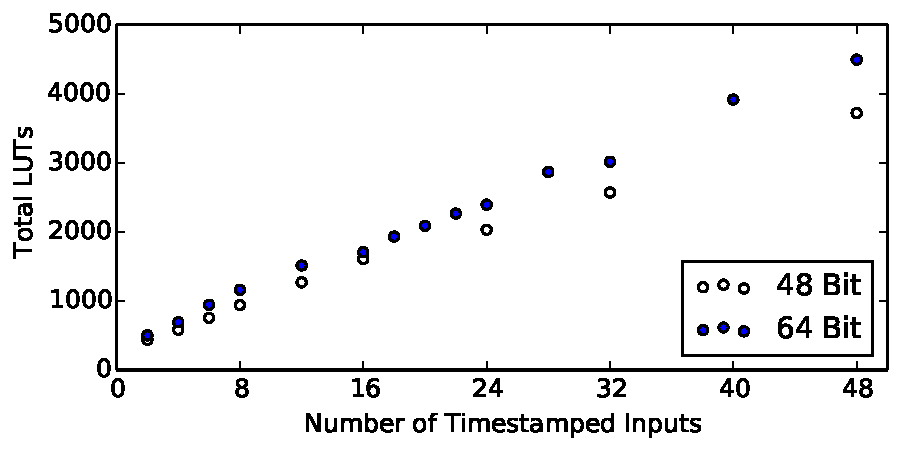
\includegraphics[width=0.75\textwidth]{figures/pdes-hub-lut-scaling.pdf}
    \caption{Measured LUT utilization, combined logic and memory, of the design hierarchy enclosed by the
    simulation wrapper as a function of timestamped input count. The main
    driver of increased utilization is the frontend of the hub unit's control
    pipeline, followed by the introduction of new message queues.}
    \label{fig:pdes-hub-lut-scaling}
\end{figure}

Another potential concern is the LUT utilization of the frontend of the hub.
In Figure~\ref{fig:pdes-hub-lut-scaling}, we report LUT utilization of all
modules under the simulation wrapper versus the length of the scan chain. This
includes the hub and channel implementations, but excludes all bridges and
FPGA-shell collateral like DRAM controllers. LUT utilization scales nearly linearly
with increasing input count with approximately 86 and 74 additional LUTs required per
timestamped input for 64 and 48 bit designs respectively. While not
insignificant, the 4494 LUTs used in the 48 input, 64-bit variant accounts for
just 0.38\% of the total available LUTs in a Xilinx Ultrascale+ VU9P.

\section{Example Case Study}

The support we've described in this chapter unlocks fast deterministic
simulation of a large space of interesting systems. In this section, we show how this
could be used to study novel thermal management and DVFS policies, by
simulating a Chipyard SoC that uses frequency throttling to stay within a
desired thermal envelope. Our system is unique among academic works in its
generality and non-invasiveness: in principle no simulation specific devices need
to be exposed to target software, and target drivers need not be modified for
FireSim since they continue to write to the same memory-mapped registers that
would be present in the actual chip. Of course, performance-accurate simulation is only
one half of this puzzle---a detailed power model is required to complete
the loop. Prior work based on FireSim, notably Simmani~\cite{Simmani}, would be
a good fit if and when it is upstreamed into FireSim.  In lieu of a more
accurate power model, we've used a simple replacement which is sufficient to
demonstrate the work described in this chapter.

\subsection{Target SoC}
Here we simulate a single-core rocket-based SoC, shown in
Figure~\ref{fig:pdes-demo-target}, which differs minimally from what one can
generate from Chipyard 1.4 out-of-the-box. While it would be easy to implement
a simple PLL TU that could step up a slower reference clock to the required
frequency, here we directly supply a high-speed reference clock that is
divided down on chip. This matches what Chipyard does by default for
software RTL simulation. We modified the divider sources to
annotate themselves when they are instantiated (as in
Listing~\ref{lst:timestamped-bridge}), and instantiated our clock source bridge
to supply the reference. Our largest clocking-related change was to introduce tile clock multiplexors which select
between the uncore clock and a fast clock that runs at two times the uncore frequency. The select for this multiplexor is driven
by a memory-mapped register bound to the periphery bus which resides in the uncore domain.

\begin{figure}
    \centering
    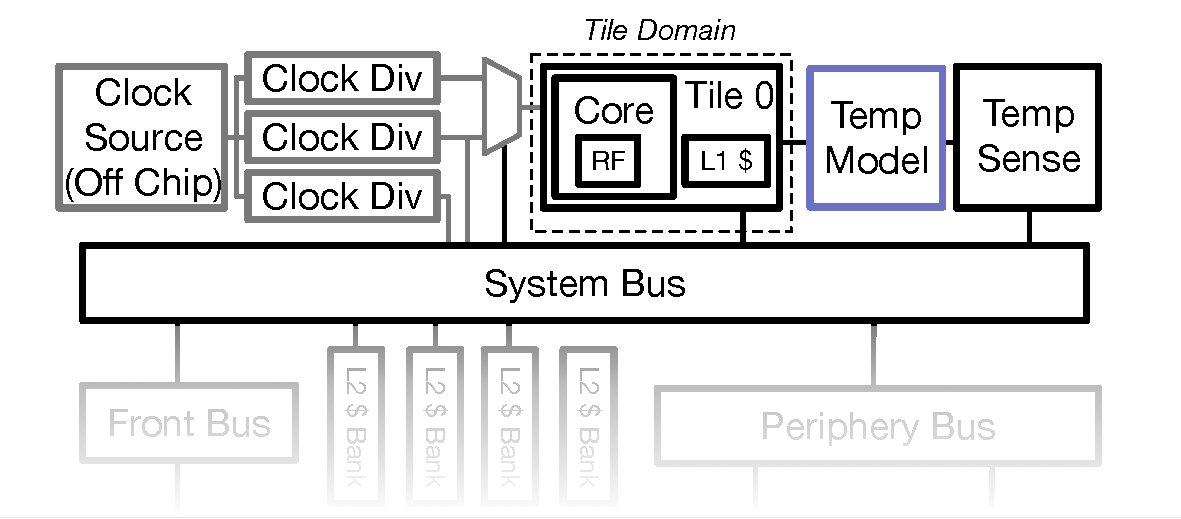
\includegraphics[width=0.99\textwidth]{figures/pdes-demo-target.pdf}
    % graffle2pdf -c pdes-demo-truncated midas-graphics/graffle/midas2-target.graffle figures/pdes-demo-target.pdf
    \caption{The modified, single-tile target used to illustrate thermal throttling. Modules in grey are
    TUs. The ``Temp Model", in blue, is a CPU-hosted bridge. It is connected to the tile's trace interface
    to measure cycle count and instructions retired, and drives an 8-bit register in the ``Temp Sense`` module.}
    \label{fig:pdes-demo-target}
\end{figure}

To integrate a temperature model, we added a temperature sensor that consists
of an 8-bit memory-mapped register fed by a CPU-hosted temperature bridge.
Target memory-mapped reads to this register return two times the current
temperature in Celsius. The bridge periodically updates this register as a
function of tile-cycles elapsed and instructions retired. To do so, the
bridge driver polls its module every $P$ uncore cycles, measures a change in
cycle count ($\Delta C$) and instructions retired~($\Delta I$), calculates an
updated temperature~($T_{new}$), and writes the updated temperature back to the target. The
temperature model selects a core voltage by adding a scaling factor proportional to $\Delta
C$ to a base. In the overwhelming majority of cases, $V$ will be either be the
base voltage or $1.5\times$ it, as the tile is unlikely to undergo a frequency
change in any given polling interval. We give the temperature model used in the bridge below:
\begin{equation}
\begin{split}
    V           & = 0.5 + \frac{\Delta C}{2P} \\
    E_{dynamic} & \propto \Delta I * V^2 \\
    E_{static}  & \propto \Delta C * V \\
    Q_{heating} & \propto E_{dynamic} + E_{static} \\
    Q_{cooling} & \propto P (T_{ambient} - T_{old}) \\
    T_{new}     & = T_{old} + Q_{heating} + Q_{cooling}
\end{split}
\end{equation}


This simple model, while completely insufficient for doing meaningful power
studies, suffices for creating regimes of high dynamic power utilization which
can will induce Linux to switch between the two operating points.

\subsection{System Software}
Practically speaking, the most time consuming aspect of building this prototype
was writing system software, since we could not reuse code from an
existing chip. While Linux provides many generic drivers that can be
configured entirely from the device tree, in the short term it was easier to write
primitive drivers as kernel modules tailored for our target. We wrote two new kernel modules,
requiring roughly 200 lines of mostly boilerplate C code:

\begin{itemize}
        % Linux version
\item A frequency scaling driver (extending \texttt{cpufreq\_driver} that binds to
Linux's \texttt{cpufreq} subsystem. \texttt{cpufreq} is the canonical mechanism for implementing dynamic
    frequency scaling in Linux. The target-specific component of this
driver supplies a table of two operating points and implements functions for
initialization, de-initialization, and frequency switching. The latter accepts an index
into the aforementioned table and writes to the tile clock multiplexor accordingly.

\item A thermal zone device driver that implements a function to read the
    device's temperature. This driver defines polling intervals, temperature
    trip points and trip types. We configured the driver polls the
    temperature sensor every 100 ms and added a single trip point set to
    40C.

\end{itemize}

Interaction between these two drivers is fairly straightforward.  When Linux
brings up the \texttt{cpufreq} subsystem during boot, it creates a new policy
backed by our custom driver. We use Linux's \texttt{ondemand} governor for this
policy, which picks the fastest available operating point unless the system is
idle. Later in boot, the thermal zone device for our temperature sensor
initializes and binds itself as a cooling device to the \texttt{cpufreq} policy
above. When the thermal zone device reads a temperature above the 40C trip point,
\texttt{cpufreq} will restrict the available operating points of the policy to
the slower frequency. When this occurs the policy is then forced to
update: it switches to the available operating point, which produces a
write to a memory-mapped register driving our clock multiplexor. When the temperature
drops below this trip point, both operating points once again become available, and so
unless the system is idle, the ondemand governor picks the faster operating
point and the clock multiplexor setting is updated.

\subsection{Demonstration}

To demonstrate the operation of this system, we booted Linux on the target
above, with our custom drivers, and ran the SPEC 2017 benchmark
\texttt{657.xz} with its smaller ``test" input. We tuned the coefficients of
our model to produce frequency transitions in the timescales of this benchmark.
Notably, we set $P = 10^6$, and $T_{ambient} = 20$C.
In Figure~\ref{fig:pdes-demo-plot}, we plot temperature~(C) and IPC versus
time. We calculate IPC in terms of the fixed uncore clock to better highlight
operating point changes: this permits rocket's IPC to reach two when running at
the faster operating point despite being a scalar core.  Regions of the graph
shaded in lavender indicate the core is running at the slower operating point;
the graph has white background otherwise.

\begin{figure}
    \centering
    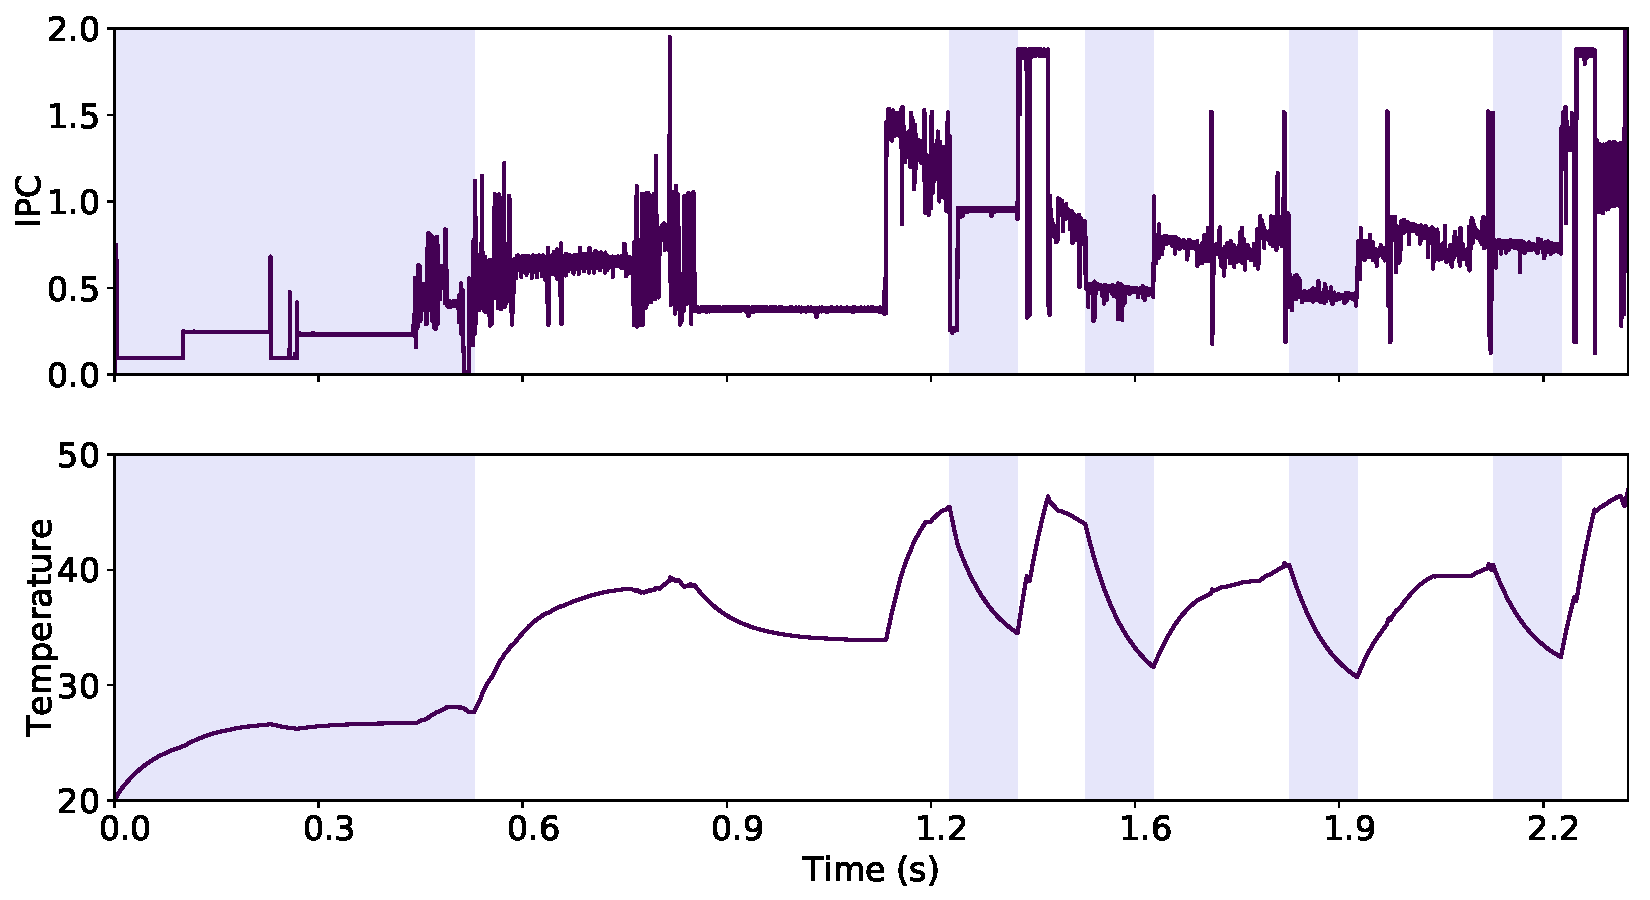
\includegraphics[width=0.99\textwidth]{figures/pdes-demo-plot.pdf}
    \caption{IPC and temperature (C) versus simulated time for \texttt{657.xz} running its 
    test input. Regions in lavender indicate the core is running at the slower operating point (uncore frequency)
    whereas regions in white indicate is core is running at two times the uncore frequency. We plot IPC and temperature sampled
    every hundred thousand cycles, and apply a ten-sample rolling average.}
    \label{fig:pdes-demo-plot}
\end{figure}

After coming out of reset, the tile starts at the slower frequency. Here it
remains until Linux brings up the \texttt{cpufreq} subsystem.  After
initialization, the governor switches to the faster operating point, producing
the first transition visible in Figure~\ref{fig:pdes-demo-plot}.  Later during
Linux boot the thermal zone device for our temperature sensor is registered,
and bound to the \texttt{cpufreq} policy above. Since the chip is not above
40 C, no frequency changes are made. Linux boot completes around
0.8 seconds into simulation time and the workload immediately starts.

The first throttling event occurs after a burst of relatively high IPC in the benchmark around 1.2 seconds. Here there is a precipitous drop in IPC
that reflects that the core frequency has been halved. After one polling
interval of the sensor, the temperature of the device has dropped sufficiently
to re-enable the faster operating point, and the policy switches back to the
faster mode. The policy performs this dance for the remainder of the
simulation, though later periods of the benchmark have relatively lower IPC which permit the chip to
run at the higher frequency longer before the core is throttled.

We ran this workload on an earlier version of our prototype that used the
baseline TUs. We measured $FMR = 12.5$ giving an $f_{emul}$ of 9.6 MHz. The
increase of FMR over the 11.0 baseline we reported in
Table~\ref{tbl:pdes-baseline-fmrs} is due to simulation stalls induced by the
temperature bridge to measure and update the core temperature.  There is no
reason this can not be overlapped with simulator execution, which would be
critical if we re-ran this experiment using the optimized TUs. Indeed, with the optimized TUs we
expect $f_{emul}$ to be close to 60 MHz---a figure approaching the throughput
achievable using prototyping-based approaches like that proposed by Mantovani et
al.~\cite{DVFSPrototype} but without many of the aforementioned limitations.

\section{Interaction with Multi-Cycle Optimizations}\label{sec:pdes-latency-overlapping}

One justification for exploring the distributed approach described in this
chapter was that a potential FMR increase may overlap with one brought about by
multi-cycle optimizations. This might hide some or all of the potential slowdown. These
optimizations increase FMR significantly because tokens must propagate between
a hub and spoke~(the same effect responsible for two cycles of latency in our
clock gate target) but, in contrast to some of our TUs, the UU
itself takes multiple host cycles to process one target cycle. Theoretically,
this means that FMR increases brought about by multi-cycle optimizations should
exceed many of the figures we reported in
Section~\ref{sec:pdes-common-circuit-perf} and
Section~\ref{sec:pdes-opt-units}.

%We leave more complete study of performance interactions to future work, as the
%interactions brought about composing our scheme with multi-cycle resource optimizations can quickly become complex. 
To illustrate this effect we measure the performance of three quad-core BOOM
simulators, one based off mainline FireSim and two using the work of this
chapter. We use the ``LargeBoom" configuration: core microarchitectural parameters match those previously shown in Table~\ref{tbl:core-parameters}.
As we reported in our ICCAD paper~\cite{GoldenGate}, this system
cannot fit on a single VU9P device\footnote{In fact, the ``LargeBoom"
configuration has grown substantially since our ICCAD publication. As of
Chipyard 1.4 only a single core will fit on the FPGA without resource
optimizations.}, so we will recruit the assistance
of the multi-cycle RAM optimization to efficiently implement BOOM's integer and floating point register files.  Note, the target RTL for the statically
and dynamically clocked systems differs only in how their clocks are generated.
All of these systems have clocks running at three distinct frequencies: a 500
MHz DRAM clock, a 750 MHz uncore clock, and
1.5 GHz tile clock. The statically clocked system uses the clock generation scheme
described in the previous chapter and fixes all four tiles at 1.5 GHz. The two
dynamically clocked systems resemble the target we used in the thermal
throttling demonstration~(Figure~\ref{fig:pdes-demo-target}:
a high-speed clock source~(1.5 GHz) feeds
parallel clock dividers to provide the uncore and DRAM clocks, and each of the
four tiles is given its own clock multiplexor. The two dynamically clocked variants differ only in
their TU selection: ones uses the lookahead-optimized units and the other uses
the baseline implementations.  All-in-all, resource utilization is
approximately the same across all designs, though the dynamically clocked
configurations use seven BUFGCEs instead of three.  All three designs closed
timing at 40 MHz.

For the pair of dynamically clocked systems, we consider two runtime operating conditions:
one in which all cores are clocked at 1.5 GHz, and one in which they are all
clocked at 750 MHz for the duration of boot. We had the first-stage
bootloader~(BBL) configure the tile multiplexors before the kernel starts. In the slower case, the RAM models are only active in every
other fast-clock cycle, providing fewer opportunities for the delays in
timestamped message passing to be hidden. As a final note, in this experiment we use the
RAM optimization first presented at ICCAD2019 and not the throughput-optimized
variant presented by A. Magyar in his dissertation. This unit statically
schedules all register file accesses thus has a fixed FMR.  A. Magyar reports an
FMR of 12.1 for ``Large BOOM" configurations using this optimization.


\begin{table}[t]
\centering
    \begin{tabular}{c c c c c c}

        &                 & \multicolumn{2}{c}{Tiles @ 1.5 GHz} & \multicolumn{2}{c}{Tiles @ 750 MHz} \\
        & \textbf{Static} & \textbf{Baseline} & \textbf{Optimized} & \textbf{Baseline} & \textbf{Optimized} \\
    \hline
          FMR            & \multirow{2}{*}{12.1} & \multirow{2}{*}{21.0}  & \multirow{2}{*}{12.1} & 16.0 & 7.0 \\
          FMR$_{tile}$     &  & & & 32.0 & 14.0 \\
          %Wallclock Time & 707.8 & 1258.8 & 721.8 & 1349.3 & 585.8 \\
    \hline
    \end{tabular}
    \caption{Measured FMR of a quad-core ``Large BOOM" SoC with the multi-cycle RAM optimization
    applied to all register files. Tile frequency in the dynamically clocked configurations
    (columns labeled with ``Tiles @ \{1.5 GHz, 750 MHz\}") was set by the first stage
    bootloader and fixed for the remainder of simulation. FMR in these systems
    is with respect to the 1.5 GHz clock regardless of frequency selection.
    FMR$_{tile}$ reports the FMR of the clock used to drive the tiles.}
    \label{tbl:pdes-opt-interactions}
\end{table}

To a first order, we expect latency overlapping to occur when two conditions are met:
\begin{enumerate}
\item Latency-critical messages propagate in the same simulator timestep where a multi-cycle UU is active.
\item The data values of the aforementioned messages do not combinationally depend on tokens generated by the UU with the longest latency.
\end{enumerate}
Since the register driving the clock multiplexor select is many cycles removed
from a register file access, the second condition is met in our designs.
Otherwise, the FMR penalties of register file access and message propagation
would be serialized. Thus, any observed slowdowns should arise because the
first condition has not been met.

We report the FMR of these configurations in
Table~\ref{tbl:pdes-opt-interactions}.  Since the timestamped subgraph in these
simulators is identical to that of the clock multiplexor organization we
studied in Section~\ref{sec:pdes-common-circuit-perf}, we would expect FMRs of
at least 11.0 and 2.0 for designs using baseline and optimized TU
implementations respectively. When running at the fast clock frequency, the
optimized clock multiplexor configuration can completely hide its FMR cost
because the negative edge is squeezed out of hub-unit pipeline while the
multi-cycle RAM model is operating (this is possible because the hub already has
a future positive edge it can schedule). Conversely, in the baseline
configuration the negative edge timestep cannot be squeezed out, since the
clock multiplexor requires a null message at that timestamp to produce the next
positive-edged message on the multiplexor-selected clock. Since the RAM model
is not active on negative edges of the tile's clock, this latency cannot be
overlapped. This produces the apparent partial overlapping observed in the
baseline configuration.

When all tiles run at the slower frequency, $FMR$ decreases but FMR$_tile$
increases in both cases, because the RAM models remain idle on every other fast
clock edge.  Note that FMR$_{tile}$ is larger than a static configuration would
be running at the same frequency (where FMR = 12.1). Here the FMR of the
timestamped subgraph is exposed directly to the simulator on every other fast
clock positive edge. Thus, adding the expected FMR of the the timestamped
subgraphs running in isolation (11.0, 2.0), to the measured FMRs of the ``Tiles
@ 1.5 GHz" case, produces the observed FMR$_{tile}$ in these slower
configurations.

The main takeaway here is that, if a TU depends only on messages in timestamps
in which multi-cycle UUs are active, their latencies can generally be
completely hidden. For example, if we were to add clock gates to the tile, the
four cycle FMR penalty would be hidden so long as at least one other core is
not clock gated. In a single-tile configuration, any cycle in which the core is
clock gated disables execution of the multi-cycle RAM unit, exposing the
clock-gate's FMR penalty of four. The expected FMR of this system would
therefore be FMR $= 4p + 12.1(1 - p)$, where $p$ is the fraction of tile clock
cycles in which the clock is gated. Naturally, these observations are closely
tied to our current implementation, specifically to that of the hub unit---in
the next section, we explore future work including some ideas that would expose
more opportunities to overlap latencies.

\section{Limitations and Future Work}\label{sec:pdes-future-work}

From the outset, the attractive aspect of our PDES-based approached, was that
it provided a flexible abstraction to inject arbitrary models of non-SSM
circuits. While it is more resource intensive then a more direct centralized approach, the
real cost of this abstraction is increased FMR.  As we showed in Section~\ref{sec:pdes-latency-overlapping}, in
some cases the latency introduced by modeling TUs can be overlapped
with the increased execution time of multi-cycle UUs---in this way, our PDES-based
approach dovetails with Golden Gate's defining feature. However, the overwhelming majority of FireSim users simulate smaller target
systems in which no optimizations are required and the expectation is that
simulators run close to unity FMR. So, for our approach to be viable, it needs to recoup the performance
losses it has introduced over the implementation described in the previous
chapter. This will require overcoming throughput bounds
that limit feedforward topologies~(e.g., clock divider trees), and more critically, the latency bounds introduced by cycles in
the timestamped subgraph.

\subsection{Overcoming Throughput Bounds}
To replace the existing clock generation in FireSim, described in the previous chapter, overcoming the
throughput bounds of feedforward networks would be sufficient, as networks of clock
sources and dividers can subsume the existing feature set.

The best case FMR of our approach is currently two because positive and
negative edges for clocks are enqueued and dequeued as separate messages. There
are a few potential fixes for this. The first is to use a better clock-message
encoding, for example, one that encodes both positive and negative edge times. This is not a panacea, because both
positive and negative edge times may not be known at enqueue time. In practice,
TUs would need to support both single and double-edged variants of clock
messages. Alternatively, for fixed clocks whose frequencies are known at the start of simulation, the
time zero message could simply encode the period and phase of the clock:
sinks would need only one message to be set for the remainder of simulation.

Even if the FMR-of-two limitation is lifted, the presence of high-frequency
reference clocks, that are not used to drive logic in the target, can introduce
a new bandwidth bound. In a system with clocks running at 1.5 GHz, 1 GHz, and
750 MHz~(as in our system described in the previous chapter), using only
integer dividers requires a 3 GHz reference clock. Even with the denser
double-edged message encoding described previously, the system would run with
FMR of two for the core domain. To improve this and support modeling
high-frequency clock generators like VCOs in \emph{independent} TUs, some form of
multi-period encoding of clocks is unavoidable.

Without this there are two simple paths forward. The first is to preclude
modeling high-frequency clock sources and downstream dividers as distinct
units, but instead fold them into a single unit.  This removes the high
frequency channel from the timestamped subgraph. Since output dividers are often integrated
into PLL IP, it would be natural to swap them out together and replace them
with a general but abstract PLL model whose implementation is optimized to
ensure high output-message throughput. In the short term, if we do not wish to
modify clock token encodings, we could configure clock dividers to assume their
inputs have fixed periods, which they would learn after receiving their first
pair of input messages.  This would permit them to look arbitrarily far ahead
of their inputs.

\subsection{Overcome latency bounds}
If there is a fundamental problem with the deadlock-avoiding approach we've
outlined in this chapter, it is that latency through loops in the timestamped subgraph
graph can substantially increase FMR. This is especially evident in the
baseline TUs. Since many
clocking primitives are tightly coupled to the rest of the target, it not
always possible to build TUs that have sufficient lookahead to hide message
transmission and hub-unit pipeline latency. This was most clearly demonstrated
with our optimized ICG, which directly exposes the four-cycle hub-TU loop
latency. Staying within the regime of using decoupled TUs, there are a few general approaches
to improving FMR.

This first is to simply cut latencies where possible. The four-cycle update
loop between the hub and a TU could be improved by using flow-through queues
between the hub unit and sink TU, shaving one cycle of latency. More aggressively, it may also be
possible to combine the first two stages of the hub's control pipeline for small numbers of timestamped inputs. Since
Vivado places all BUFGCEs in the same clock region as the main simulator clock
(to produce balanced trees), there may be little benefit to having the extra
stage as there is insignificant routing delay from the stage-1 registers to the
clock buffers. Both of these ``fixes" have the potential to decrease
$f_{fpga}$, and may not be universally applicable.

A more intelligent messaging encoding and channel implementation is also worth
exploring.  Currently, null messages occupy slots in the channel queues. This
may produce head-of-line blocking where a TU is forced to dequeue a null
message before it can observe a real transition, potentially adding an extra
cycle of latency. Ideally, these extraneous null messages would be squashed
out.  In practice there is no need to enqueue null messages, instead, the
channel could update a secondary time register whose value would always match
or exceed the timestamp of the non-null message at the head of the queue. When
any new message is enqueued this value is increased. Null messages could then
be dropped with no loss of information.

Some other approaches which we have not previously mentioned in earlier in sections include:
\begin{itemize}
    \item Introducing global optimizations that would share information about
        source behavior to sinks.  The example from the previous section where
        a clock divider may assume its input is fixed is one example of this.
\item Allowing hub-unit output channels to decouple. If a clock domain has just
    fired, timestamped outputs affected by transitions in that domain likely
    are not going to change in the near future. This information could be
    captured in first output message, instead of waiting for additional
    timesteps to issue new null messages.
\end{itemize}

\subsection{Future Work, Performance Aside}

Working within the PDES abstraction laid out in this chapter there are many other avenues, beyond performance optimizations,
worthy of consideration:

\begin{itemize}
\item Build out a larger library of optimized TUs. Notably absent from this chapter
is a PLL TU. Here, it would be relatively easy to build a simple model with
integrated output dividers. This could be expanded to include a laundry
list of other features, including modeling locking time and supporting
fractional output dividers. As previously mentioned, all of this could be
done without exposing the high-frequency VCO output to the simulation graph.

\item Add asynchronous reset to existing TUs. For this to perform well, the asynchronous-reset
message stream will need to lead other inputs (which may be
difficult to ensure), or the TU will have to find asynchronous-reset relative
lookahead, which generally speaking is not possible. Here the designer could artificially
introduce lookahead if they know that asynchronous-reset-launched transitions
can be safely be ignored such that they may be delayed.

\item Explore automatic translation of verilog to TU implementations. Writing complex
TUs can be difficult. This would sidestep that challenge and produce models
that, ideally, faithfully represent the source (once the tool itself has been verified). For this to work well, the compiler must
find lookahead opportunities that span the circuit.

\item If bespoke TUs are required for high performance having a better strategy for
verifying them against a reference becomes crucial. For the same reasons LIME
was effective for verifying primitive LI-BDNs, an equivalent model checking flow
would be useful for TUs. Simulator deadlock avoidance could be guaranteed by
proving a TU implementation has non-zero lookahead. Checking message
correctness would be be considerably more difficult.

\item Integrate an accurate power model. In providing RTL-faithful timing
    accuracy, the infrastructure outlined in this chapter unlocks a critical
    piece of doing accurate research on novel DVFS-capable systems.  Adding
    a power model, tailored for the target, would make FireSim a compelling framework for doing full-stack DVFS research. Here, integrating
    Simmani~\cite{Simmani} is the obvious next step\footnote{A snapshot
    and replay approach like Strober's is also tractable but considerably
    more challenging to get working under Golden Gate due to increased
    simulator complexity.}. This would only require a new target transformation, to wire up signals of interest
    as selected by Simmani to a custom bridge, and no internal modifications to Golden Gate.
\end{itemize}

%With optimized TUs producing $f_{emul}$s in the range of 10-80 MHz, this
%infrastructure runs many orders of magnitude faster than software-based
%techniques used for evaluating these systems. Necessarily, many software based
%schemes use simulator specific drivers~\cite{gem5dvfs}, which our approach
%skirts by using silicon-realizable RTL and modifications RTL that in many cases
%need not be visible to target software.  Moreover, our scheme execution rate
%falls within an order of magnitude of the FPGA prototyping-based infrastructure
%proposed by Mantovani et al.~\cite{DVFSPrototype}, while making fewer
%assumptions about both the target and host system.  Unlike that work, our
%design should be trivial to port to different Xilinx and Intel FPGAs in the
%future since it relies only on clock-gating to produce derived clocks. While
%FireSim is generally used with Chisel-generated designs, there is nothing
%funamdentally precluding the emission of FIRRTL from a different design
%language, or translation of Verilog into FIRRTL, dramatically expanding the
%scope of designs our system is capabale of simulating.


%\subsection{Alternative Approaches}
%
%While some combination of the aforementioned optimizations would undoubtably
%improve simulation FMR, they would could dramatically increase simulator
%complexity, they have their limits. The reality is that closely coupled
%clock-generating circuits, like ICGs and clock multiplexors, are probably best simulated \emph{in
%situ}, instead of being extracted into a decoupled unit. State for these
%circuits can be left in the target, and combinational functions they perform on
%clocks can be hoisted into the hub-unit's second stage to act on future clock
%enables. This would generate new clock buffers for these derived clocks. This clearly would be
%insufficient for modelling clock generators, that can't be described as digital functions on existing clocks, like PLLs.
%For modelling this class of circuits, having an indepedent unit seems entirely sensible.


%\section{Deadlock Considerations}

%Patents:
%https://patents.google.com/patent/US20150046144A1/en
%
